\documentclass[conference]{IEEEtran}

\usepackage[dvips]{graphicx}
\usepackage{graphicx}
\usepackage{amsmath,amssymb}
\usepackage{algorithm}
\usepackage{algorithmic}
\usepackage{flushend}
\usepackage{cite}
\usepackage{pdfpages}

\begin{document}
\title{Different every time: A framework to model real-time instant message conversations}
\date{}%date stay empty

\author{\IEEEauthorblockN{Jonathan Dunne}
\IEEEauthorblockA{Hamilton Institute\\
Maynooth University\\\
Email: jonathan.dunne.2015@mumail.ie}
\and
\IEEEauthorblockN{David Malone}
\IEEEauthorblockA{Hamilton Institute\\
Maynooth University\\
Email: david.malone@nuim.ie}}\maketitle

\begin{abstract}
As startups and micro teams adopt real-time collaborative instant messaging solutions, a wealth of data is generated from day to day usage. Making sense of this data can be a challenge to teams, given the lack of inbuilt analytical tooling. In this study we model the distributions of duration, inter-arrival time, word count and user count of real-time electronic chat conversations in a framework, where these distributions can be used as an analogue to service time estimation of problem determination. Using both an enterprise and open-source datasets, we answer the question of what distribution family and fitting techniques can be used to adequately model real-time chat conversations. Our framework can help startups and micro teams alike to effectively model their real-time chat conversations to allow high value decisions to be made based on their collaboration outputs.
\end{abstract}

\section{Introduction}

Real-time collaboration solutions are being marketed as a way for teams regardless of size of to increase their productivity \cite{SmartCollab} \cite{eightbiz} \cite{slackSME}. One of the benefits of using such software is that conversations are segmented into either spaces, channels, or chat rooms which facilitate discussion in a linear fashion. As all conversations are recorded, rolling back to prior conversations can be done with the spin of a mouse wheel or the swipe of a screen. High end collaboration suite also include an additional set of features such as a file repository, knowledge management software and ability to screen share.  A number of feature rich solutions include: Watson Workspace \cite{WatWork}, Slack \cite{Slack}, Microsoft Teams \cite{MSTeams} and Azendoo \cite{Azendo}, to name but a few.  

One of the key selling points of of real-time collaboration suites is the idea that real-communication reduces the need for email communication \cite{emailclutter}, thus solving the problem of `email paralysis' \cite{emailparal} which is the effect of having such a large volume of email an individual is unable to communicate due to the sheer volume of messages. However both micro-teams and startups face new challenges with the adoption of real-time collaboration software. As usage increases over time, so does the volume of data. Furthermore as current offerings offer little in the way of in-built analytical solutions, making sense of the growing volumes of collaboration data is key.  

While micro-teams and startups have a number of key usecases, a growing trend is for development teams and DevOps alike to use real-time collaboration software to facilitate their ability to debug problems, otherwise known as problem determination \cite{devslack} \cite{devopsslack}. The time to debug and fix a problem is typically defined as the service time and the time between successive problems is known as the inter-arrival time \cite{kleinrock1975queuing}. By a logical extension we can see that the duration of a group chat conversation and the time between the start of such conversations could be referred as an analogue to service time and inter-arrival time duration respectively. Modelling such data may give us greater insight in a teams ability to solve problems. \par 

In this paper we propose a framework that both startups and micro teams can use to effectively model their group chat instant messaging conversations using a number of available techniques. The core idea of this framework is for small teams to use the output of modelled conversations to gain insight into the expected time of a group chat and once a conversation has completed when the mean time until the next conversation begins. For startups and micro teams with a limited team size, understanding the duration of a group chat conversation can aid problem resolution outcomes. \par

This study contains research conducted on two large real-time chat discourse datasets. Our first dataset is an enterprise dataset from a real-time collaboration application, our second dataset is an open source data set from an internet chat relay (IRC) channel. Through study of this data we investigate what techniques can be employed to effectively model the distributions of chat duration, interval, inter-arrival time, the number of words per chat conversation and the number of  users per single chat conversation. Using the results of this study for our framework, a modelling suite can be developed to provide teams with a greater level of introspection of their chat data. \par

The rest of the paper is structured in five sections: Section II provides a description of background and related works. Section III describes the both datasets as well as our method and approach. Section IV provides analysis of our experiments. It is followed by section V that explains our results. Finally, the conclusion and future work are described in section VI. \par

\section{Background and related research}

\subsection{Distribution Fitting}

Probability distribution fitting is the fitting of a known probability distribution to a data set regarding the repeated measurement of a variable phenomenon. The type of fitted distribution can vary depending on the under lying data set. The main purpose of distribution fitting is to predict the probability or to forecast the frequency of occurrence of the magnitude of the phenomenon in a certain interval.

There are two main fitting techniques used. The first method is called the method of moments. This method uses expected values of a random variable (a moment) from a population. A sample is then taken from the population and subsequent moment is estimated. The sample moments are used to make estimates about an unknown population. This idea was first proposed by 
Karl Pearson in 1894\cite{pearson1894contributions}.

The second method is called Maximum likelihood estimation (MLE). MLE is a method to estimate the the parameter values of a model by determining parameter values that maximise the likelihood.  This method was first proposed by Ronald Fisher in the 1920's \cite{fisher1925theory}, with a subsequent formal proof by Samuel Wilks in 1938 \cite{wilks1938large}.

\subsection{Goodness of Fit Testing}

If a suitable probability distribution can be found to fit a data set, of interest is how well the distribution fit that data. A number of methods have been developed to assess the goodness of fit of a distribution to a data set. We shall discuss three of the main tests briefly.

The Cram\'er--von Mises criterion \cite{cramer1928composition}\cite{von1928statistik} is a non-parametric test which examines the goodness of fit of a cumulative distribution function (CDF) compared to that of an empirical density function (EMF). Using a significance test we can test a hypothesis of whether a data set is drawn from a given probability distribution

The Kolmogorov--Smirnov \cite{smirnov1948table} test quantifies a distance between the an EMF of the sample and the CDF of the reference distribution, or between the EMF of two samples. The idea being that the closer the distance between the two, the better the fit. 

The Anderson--Darling \cite{anderson1954test}\cite{anderson1952asymptotic} test is a statistical test of whether a given sample of data is drawn from a given probability distribution. This test is a modification of the Kolmogorov--Smirnov test as it gives more weight to the tails of data. 

\subsection{Heavy Tailed Estimation}

In probability theory, heavy-tailed distributions are distributions whose tails are not exponentially bounded. In fact these distributions have much heavier tails, for example a Pareto or Generalised extreme value distribution. For such distributions a tail index, which is essentially the shape parameter of a distribution can used used to make inferences about the underlying data. 

Hill\cite{hill1975simple} proposes one of the first methods to infer tail behaviour of a distribution function. This work is valuable in that no prior assumption of the type of distribution is required prior to inference. His tail estimation technique is one of the standard methods for measuring the index of a heavy-tailed distribution.

Pickands\cite{pickands1975statistical} provides a method to make inferences about the tail of a probability distribution function. This method can be applied to all continuous distribution functions. Pickands method is an alternative method to calculate the index of a heavy-tailed distribution.

Nair et al.\cite{nair2013fundamentals} discuss the idea that heavy-tailed data and their corresponding distributions are a more common occurrence. They also discuss various techniques to model distributions from heavy-tailed datasets.

\subsection{Hurdle Distribution}

Hurdle distributions are a class of distributions for count data that can help manage data sets with a large number of zeros or a count dataset which is exhibits either over-dispersion or under-dispersion. Mullahy\cite{mullahy1986specification} proposes the idea of a hurdle model which provides a more natural means to model over or under-dispersed count data. 

\subsection{Kernel Density Estimation}

For datasets which do not fit a known distribution family, a non-parametric approach can be taken. One such approach is Kernel Density Estimation (KDE). In KDE, a range of kernel (weighting) functions are applied to a dataset plotted as a histogram. The kernel functions are divided into various widths (bandwidth). The goal is to choose the most appropriate kernel bandwidth and function shape that best fits the histogram. Both Rosenblatt\cite{rosenblatt1956remarks} and Parzen\cite{parzen1962estimation} are credited with creating KDE in it's current form. \par

A number of significant contributions in this area have also been made in the field of KDE. These are discussed briefly.  

Kernel performance is measured by either the mean integrated squared error (MISE) or the asymptotic mean integrated squared error (AMISE). Epanechnikov \cite{epanechnikov1969non}, proposed a parabolic shaped kernel that minimises AMISE and is therefore optimal. Kernel efficiency is now measured in comparison to the Epanechnikov kernel.

Silverman \cite{silverman1986density} proposes an improved method for bandwidth selection. In his study, if a Gaussian basis function is used to approximate univariate data, and if the underlying density is Gaussian, the optimal choice for the bandwidth parameter is the standard deviation of the samples. This method is known and Silverman's rule of thumb or the Gaussian approximation. 

Sheather and Jones\cite{sheather1991reliable} provided an improved method for data-based selection of the bandwidth in KDE. Their paper included a new bias term in their bandwidth estimate, that provides good performance for a broad set of cases.

\subsection{Other related studies}

Dewes et al. \cite{dewes2003analysis} conducted a study to better understand network traffic dynamics by examining Internet chat systems. While their main research output was to demonstrate how to separate chat traffic from other Internet traffic, the authors conducted analysis of the inter-arrival times of chat messages. The authors hypothesis was as follows: Are the inter-arrival times of chat messages consistent with an exponential distribution? The hypothesis was rejected due to lack of evidence, however they found the inter-arrival times were more consistent with a heavy-tailed distribution.

Lukasik et al. \cite{lukasik2015modeling} modelled time series data of tweets to understand if a reliable prediction model could be derived to predict future tweets. Their research found that by employing a log-Gausian Cox process a higher degree of predictive precision could be achieved. The authors also found that mining text from tweet messages can improve inter-arrival time prediction.

Vande Kerckhove et al. \cite{vande2015markov} provided research into the field of inter-arrival times of electronic communication. The authors investigated the the level of inter-event dependence between postings and whether a Markovian process would be suitable to model the memory effect observed in inter-arrival online activities. For their study the authors social media data from Twitter and Reddit. Their research concluded that by allowing dependence between message wait times allows for more precise modelling than by fitting against a power-law distribution alone.

Markovitch and Krieger \cite{markovitch2000nonparametric} compared the nonparametric estimation of the probability density function of long-tailed distributions from internet based traffic against existing parametric methods. The authors found that a neither a Pareto nor an exponential model was a suitable fit to their underlying data. Additionally by using both a Parzen--Rosenblatt kernel and a histogram of variable width (a polygram) a more suitable fit was achieved.

Maioroda and Markovitch \cite{maiboroda2004estimation} discuss the nonparametric estimation of a heavy-tailed probability density function by a variable bandwidth kernel estimator. The authors discuss two approaches: A preliminary transformation to provide an information estimation of tail density and a the discrepancy method based on the Kolmogorov-Smirnov statistic to evaluate the bandwidth of the kernel estimator. The authors use internet based traffic to validate their models.

Wang \cite{viztweettimes} presents a how-to article on visualising the inter-arrival times of tweets. Using the R programming language the author describes the process to collect, visualise and determining if the inter-arrival times can be modelled by a Poisson process.

% Not sure this reference is relevant
%Priedhorsky \cite{priedhorsky2014inferring} et al. propose a content based model to estimate the location of tweet postings using a %gaussian mixture model. The authors demonstrated that their models are time-invariant.

% Not sure this reference is relevant
%Ahmed et al. \cite{ahmed2013hierarchical} present a paper for an integrated model for location and social media message content. The %authors present a framework that can be used to predict the locations of label messages.

\section{Data set}

Inter-arrival time modelling of social and collaboration message data has been shown to provide a useful way to make inferences about the underlying structure of message data. By combining prior research with our proposed framework can allow startups and micro-teams to infer the expected duration of chat conversations. This output can effective analogue to service time determination. 

The study presented in this paper examines approximately 540 real-time chat conversations from two datasets. A number of points related to each dataset are summarised in Table~\ref{tab:dataset}. 

\begin {table*}[]
\caption {Summary of dataset metrics and factors} 
\label{tab:dataset}
\begin{center}
\begin{tabular}{p{2.1cm} | p{2cm} | p{2cm} | p{1.7cm} | p{2.2cm} | p{1.8cm} | p{2.5cm}} \hline \bf{Dataset} & \bf{Total No. Messages} & \bf{Duration (dd:hh:mm:ss)} & \bf{Conversations Annotated} & \bf{Mean No. Messages per Hour} & \bf{No. Entangled Conversations} & \bf{Entangled Conversation Ratio}
\\ \hline Ubuntudev-IRC & 4223 & 3 days, 14 hours, 15 mins 0 secs & 231 & 49.10 & 57 & 0.25
\\ \hline Enterprise Instant Message chat system & 3261 & 200 days, 21 hours, 38 mins and 53 secs & 312 & 0.68 & 27 & 0.09
\\ \hline
\end{tabular}
\end{center}
\end{table*}

The first dataset analysed was the open source Ubuntu dev IRC channel. \cite{irclogs} For our study we reviewed approximately 4200 messages. For each message we reviewed whether a subsequent message was part of an existing conversation or part of a prior or subsequent conversation. For each unique conversation identified we assigned a numeric topic ID. As part of the review phase we annotated 231 unique conversations. The total time period analysed was approximately 86 hours. 

The second dataset analysed was from enterprise instant message chat system which discussed cloud infrastructure problems. For our study we reviewed approximately 3200 messages. For each message we reviewed whether a subsequent message was part of an existing conversation or part of a prior or subsequent conversation. For each unique conversation identified we assigned a numeric topic ID. As part of the review phase we annotated 312 unique conversations. The total time period analysed was approximately 4820 hours. 

In an ideal world a chat conversation will start, progress then reach a logical conclusion, however on occasion an unrelated message will be injected into an existing chat conversation. We found a number of heterogeneous chat messages which appeared mid way through a homogeneous chat conversation. We enumerated these `entangled chat conversations' \cite{elsner2010disentangling} in total 57 of the chat conversations from the Ubuntu IRC dataset and 27 conversations from the enterprise dataset were found to be entangled. It should be noted that chat disentanglement is beyond the scope of our study and will not be discussed further.

This study aims to answer the following questions. First, can the duration of our annotated chat conversations be modelled by a parametric method? If not can a non-parametric method be used? Second, can the durations between annotated chat conversations be modelled by a parametric method? If not can a non-parametric method be used? Third, what is the most appropriate method to model the inter-arrival times of chat conversations? Fourth, what modelling techniques can be used to model the number of words and lines of text in a chat conversation? Fifth, to model the number of users present in a chat conversation, is a Poisson model appropriate?

\subsection{Conversation duration modelling}

Conversation duration is defined as the timestamp of the last message in a conversation subtracted by the timestamp of the first message in a conversation. A number of conversations were recorded as being zero minutes in length, this is due to a number of short (five messages or less) conversations completing in less than one minute. 

%A small (one minute) constant was added to all conversation duration times, this would ensure fitting against distributions which support values greater than zero (e.g. Pareto)

Measuring the conversation duration is useful exercise in that given many teams use real-time chat collaboration software to discuss and debug problems, we can use the conversation as an analogue to measure service times.

Probability distributions are used in many fields to understand how likely it is for an event to happen. In the case of chat conversation duration times, our starting point is to conduct a parametric test to determine if a known distribution can be fitted to our data set. The benefit of attempting to fit a known distribution is that, if such a fit can be found, we can gain access to the mathematical properties of such a distribution (i.e. mean, variance, probability density function, cumulative density function etc.). 

When parametric methods fail to yield a useful result, additional methods are employed (i.e. Distribution body and tail modelling, Hurdle methods and non-parametric methods such as KDE)

For distribution fitting, we used the R package fitdistrplus \cite{fitdistrplus} to fit various distributions to our dataset. To validate the efficacy of each distribution,  the authors used the R package ADGofTest \cite{ADGoF}, which uses the Anderson-Darling goodness-of-fit test, to determine if the observed data follows a specific distribution \cite {anderson1952asymptotic}.

\subsection{Conversation delta time modelling}

Conversation delta time is defined as the time duration between chat conversations. For example the timestamp of the starting message in a second conversation is subtracted by the timestamp of an ending messaging in a first conversation. It should be noted in the case of an entangled conversation,  a conversation delta is recorded by a negative time value. While this may seem counterintuitive, our reasoning is that while we had a mechanism to record the number of entangled conversations we also needed to measure the level of entanglement in terms of time. By using negative time we can in effect determine at the glance which conversations are entangled.

Measuring and modelling conversation delta times can surface the waiting time between prior and future discussions. These results can help answer questions around the expected time between conversations. 

Due to the complex nature of the underlying data set (i.e. a mixture of logical conversation durations (positive durations) and entangled (negative durations)) Two approaches were considered. The first was to split the dataset into two smaller subsets, one subset contained the positive durations and second subset contained the negative durations. For distribution fitting we used the absolute values for the entangled conversation subset. The second approach was to conduct KDE modelling on the entire conversation duration dataset. 

The approach to distribution fitting and validation is the same as described in the previous subsection. Our approach to conducting a non-parametric test (KDE) to model the entire delta duration (both logical and entangled) was conducted using the R package Density \cite{Rdensity}. 

\subsection{Conversation inter-arrival time modelling}

Conversation inter-arrival time is defined as the time duration between the start of a first chat conversation and the start of a second chat conversation. In other words, the inter-arrival time is essentially the product of conversation duration plus conversation delta time.  

Measuring and modelling the inter-arrival time conversation is beneficial.  The inter-arrival time is an important component, when combined with conversation duration modelling the result can be used for to predict conversation busy and free times as part of a wider queue framework.

The approach to distribution fitting and validation is the same as described in the previous subsections. 

\subsection{Conversation message \& word modelling}

A key component of any group chat conversation are the number messages that are required to complete a conversation and the amount of words used. Performing analysis on both variables can initially tell us if a distribution can be fitted to the underlying data. If a suitable distribution can be found, this result can help answer questions such as the expected number of lines and words in a chat conversation.

Thereafter additional inference can be conducted such as topic and keyword analysis. However both topic and keyword analysis is beyond the scope of this current work and will be discussed in reference to future work in the conclusion.

Our approach to distribution fitting and validation is the same as described in the previous subsections. 

\subsection{Conversation user count modelling}

Conversation user count is defined as the number of unique users that contribute at least one message to a group chat conversation. 

Like previous sections if a suitable distribution can be found to fit user count data, this result can assist teams in determining the expected number of participants per chat conversation or the proportion of conversations that contain n number of users.  

As we are dealing with count data our initial approach will to determine if a Poisson distribution is a suitable fit to our user count data. If there is sufficient evidence to suggest a lack of fit, a test for over dispersion and under dispersion will be conducted. If there is evidence to suggest some level of dispersion within our data, we shall employ a method of hurdle modelling. This model will then be tested for goodness of fit.

To validate the goodness-of-fit of a Poisson distribution, the authors used the R package vcd \cite{Rvcd}, which uses the Chi-Squared goodness-of-fit test, to determine the level of dispersion in our count data we used the R package AER \cite{RAER}.

\subsection{Limitations of dataset}

The dataset has a number of practical limitations, which are now discussed. The process of aggregating chat messages into a cohesive conversation is a subjective one. While every effort was made on the part of the authors to align messages to a thread we accept that the process is subjective. Additionally the post times for the Ubuntu chat were measured in hours and minutes only. As a result conversation duration, delta and inter-arrival times were recorded to the nearest minute, whereas for the enterprise data set, these times were recorded to the nearest second. \par

The chat conversations that form part of this study are from a) a Ubuntu IRC developer channel and b) from an enterprise chat messaging system that discussed cloud infrastructure problems. As a result our analysis may not be relevant outside of these fields. \par

\section{Results}

We now explore the results of our analysis. A Table II contains a a summary of the results for easy reference.

\subsection{Conversation duration modelling}

Fig. 1 shows a probability density function histogram for the enterprise dataset. A total of 55 conversations were found to be of 0 minutes in length (i.e. conversations that were started and completed in less than 1 minute). These values were removed from the dataset and a Weibull distribution was found to be best fit for the remaining 257 samples. An Anderson--Darling test statistic and p-value were computed as 1.1 and 0.31 respectively. The p-value is above the 0.05 significance interval. 

\begin{figure}
\begin{center}
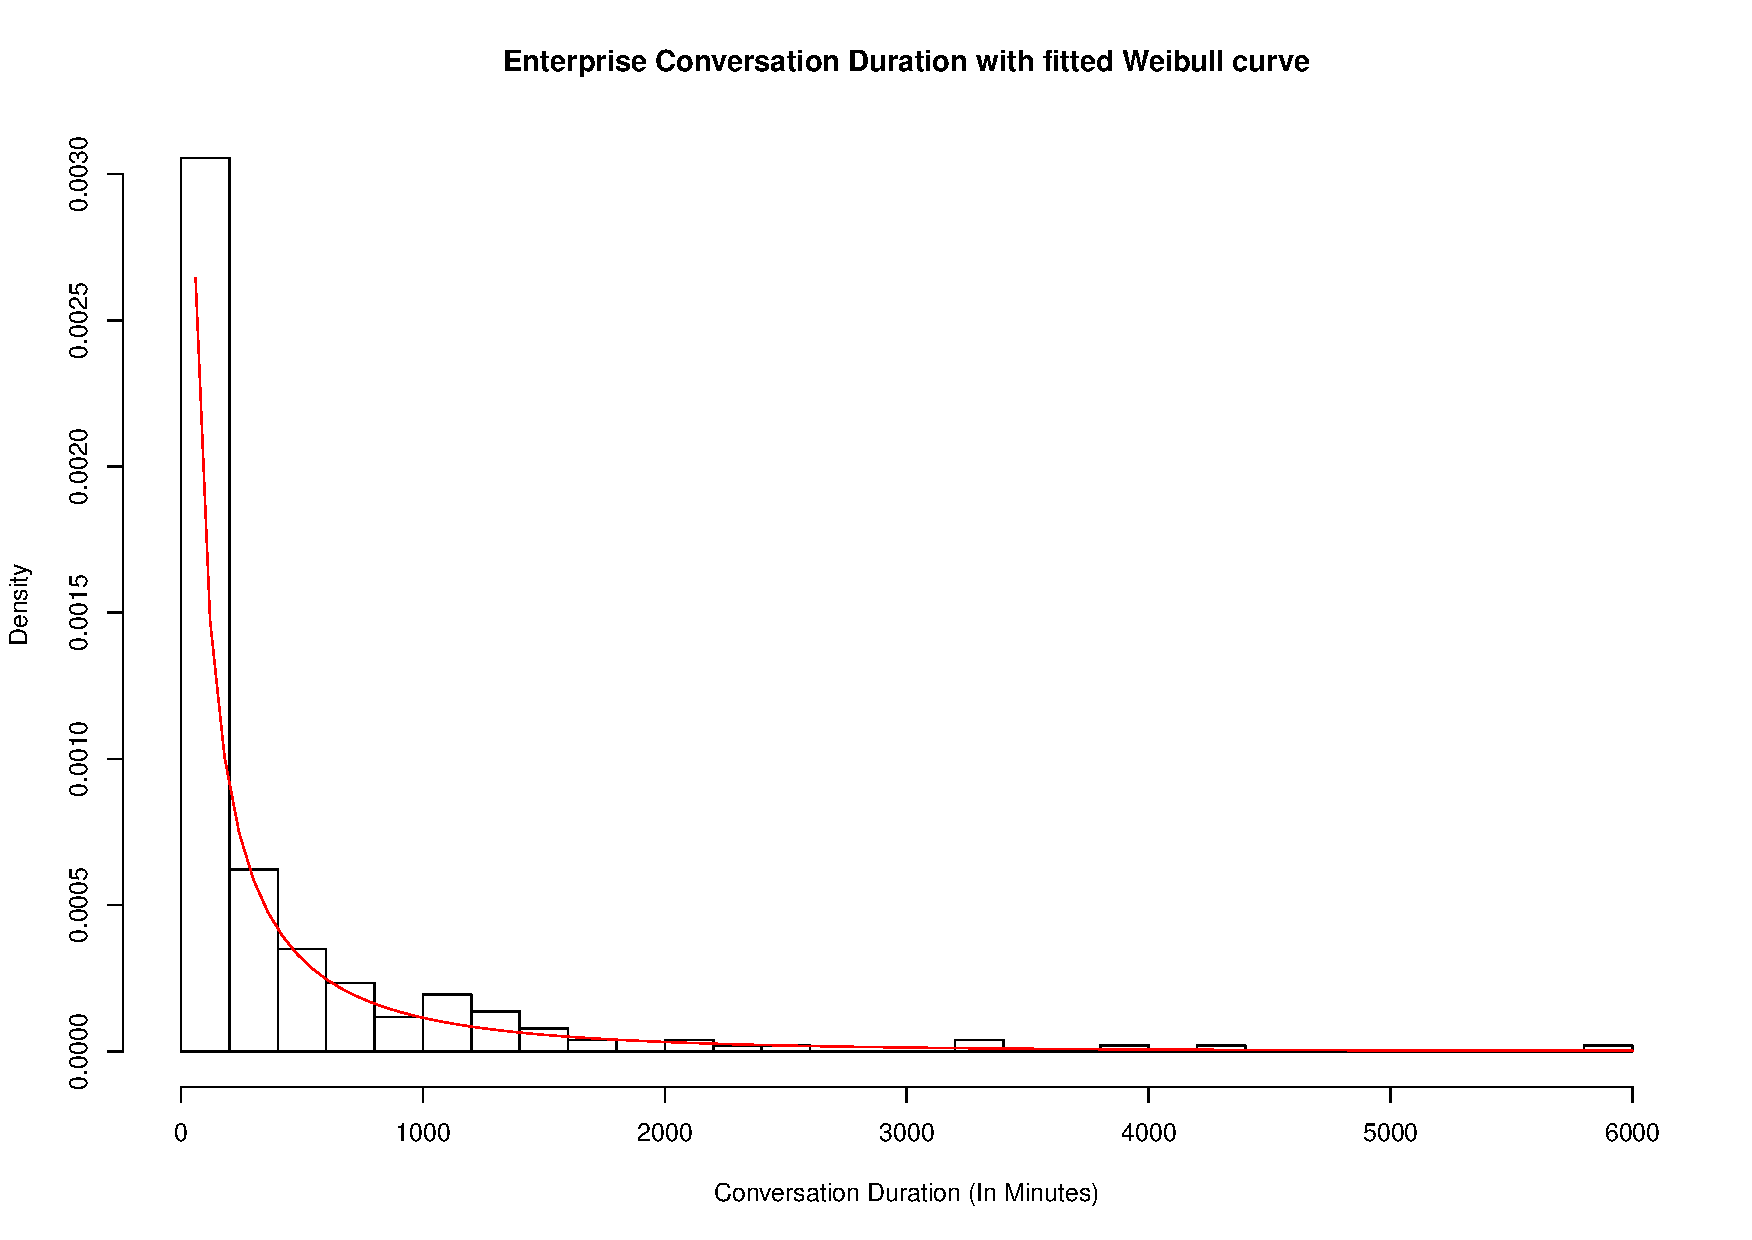
\includegraphics[height=9cm, width=9cm]{01_duration_enterprise.pdf} 
\caption{Enterprise conversation duration with fitted Weibull curve}
\end{center}
\label{fig:duration_ent}
\end{figure}


Fig. 2 shows a probability density function histogram for the ubuntu dataset. For this dataset 39 conversations were found to be of 0 minutes in length. Once again these values were removed from the dataset. Both a Burr & log-logistic distribution were found to be the best fit for the remaining 192 samples. An Anderson--Darling test statistic and p-value were computed for both distributions as 1.3 and 0.61 respectively. The p-value is above the 0.05 significance interval.

\begin{figure}
\begin{center}
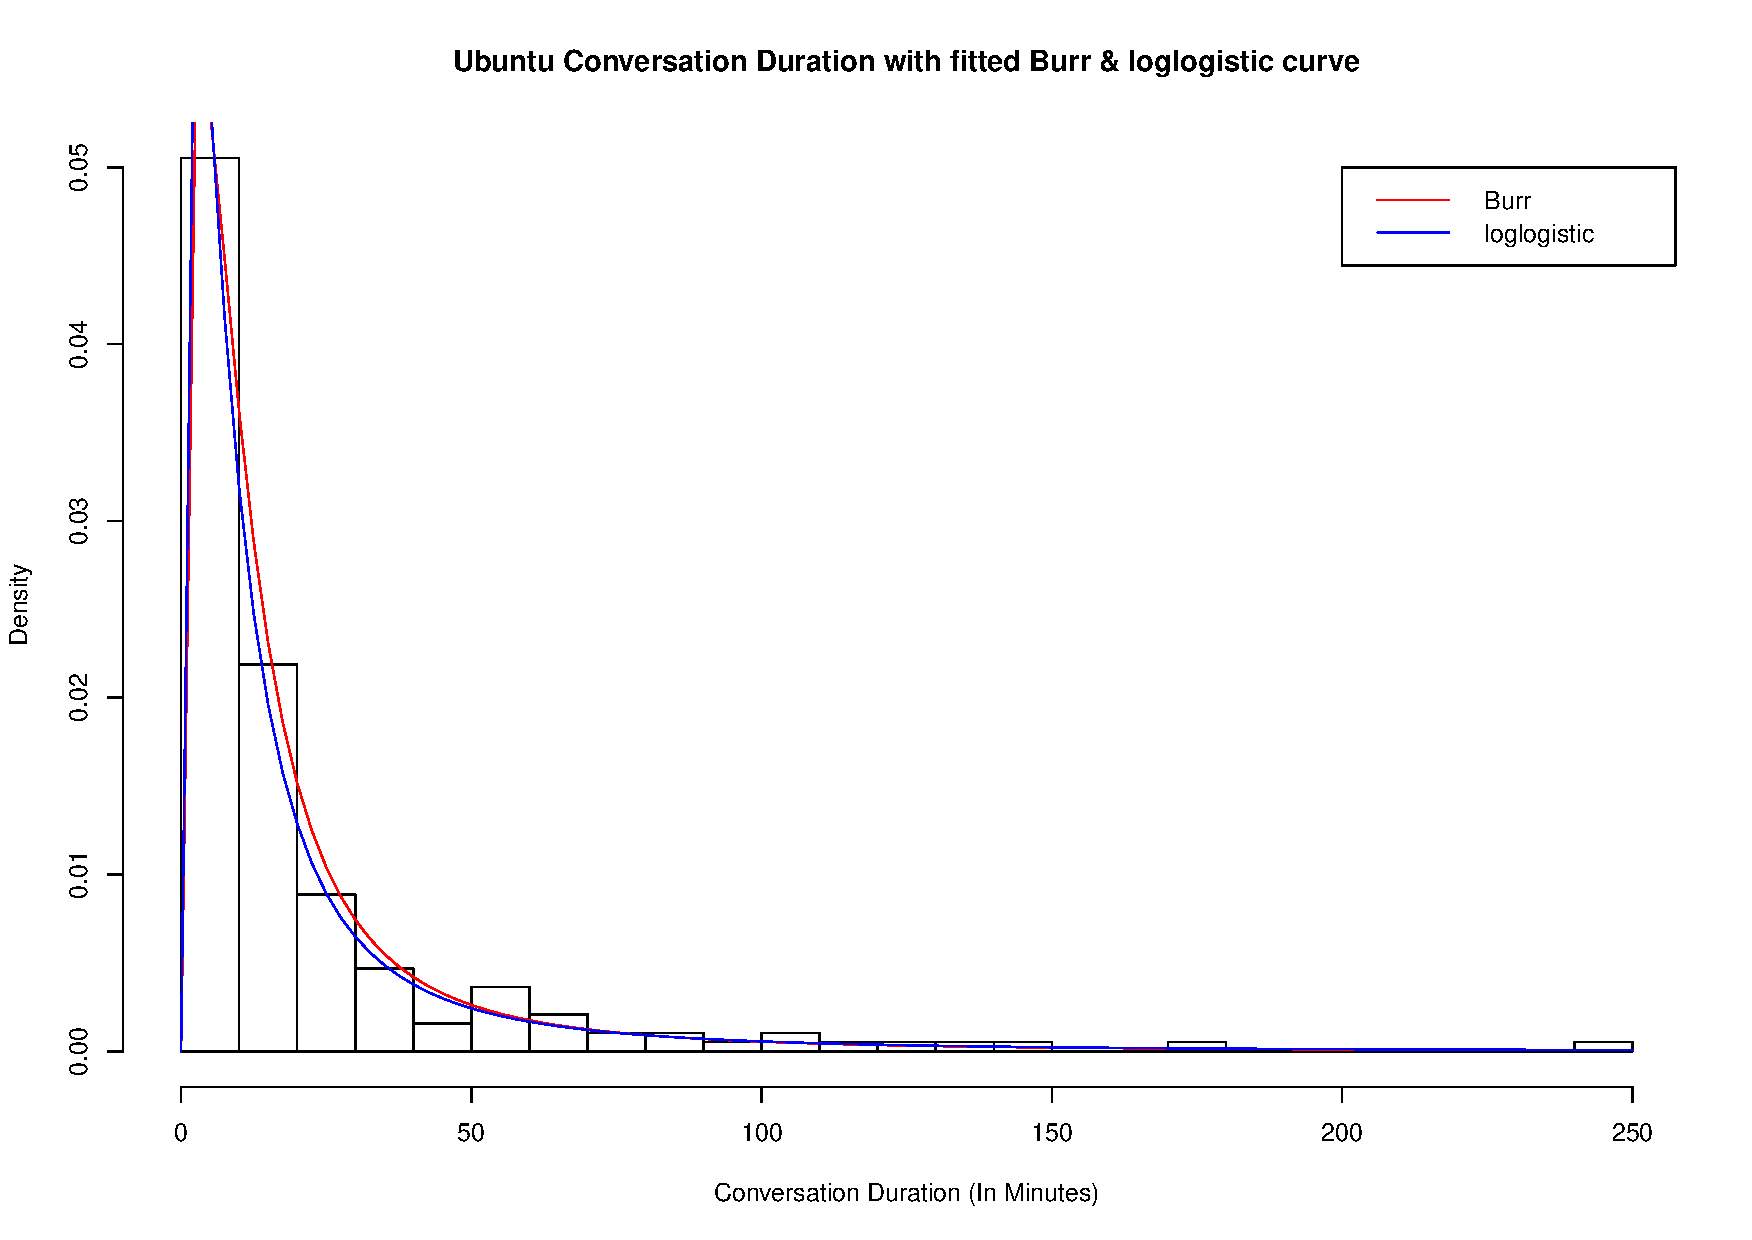
\includegraphics[height=9cm, width=9cm]{02_duration_ubuntu.pdf} 
\caption{Ubuntu conversation duration with fitted Burr & loglogistic curve}
\end{center}
\label{fig:duration_ubun}
\end{figure}


\subsection{Conversation delta time modelling}

The conversation delta time modelling results are split into two parts. The first is a parametric approach using MLE. In this approach the conversations were divided into two subsets: logical conversations (i.e. time duration between the end of an nth and the start of an nth+1 conversation, which is positive), and entangled conversation (i.e. time between the end of an nth and the start of an nth+1 conversation, which is negative). The second approach is a non-parametric approach using KDE.

Fig. 3 and Fig. 4 show probability density function histograms of both the entangled and logical conversation delta times for the enterprise dataset.  A Weibull distribution was found to be the best fit for both sub datasets.  An Anderson--Darling test statistic and p-value was computed for both distributions as 0.49 \& 0.76 (logical dataset) and 0.3 \& 0.94 (entangled dataset). In both cases the p-value was found to be above the 0.05 significance interval.

\begin{figure}
\begin{center}
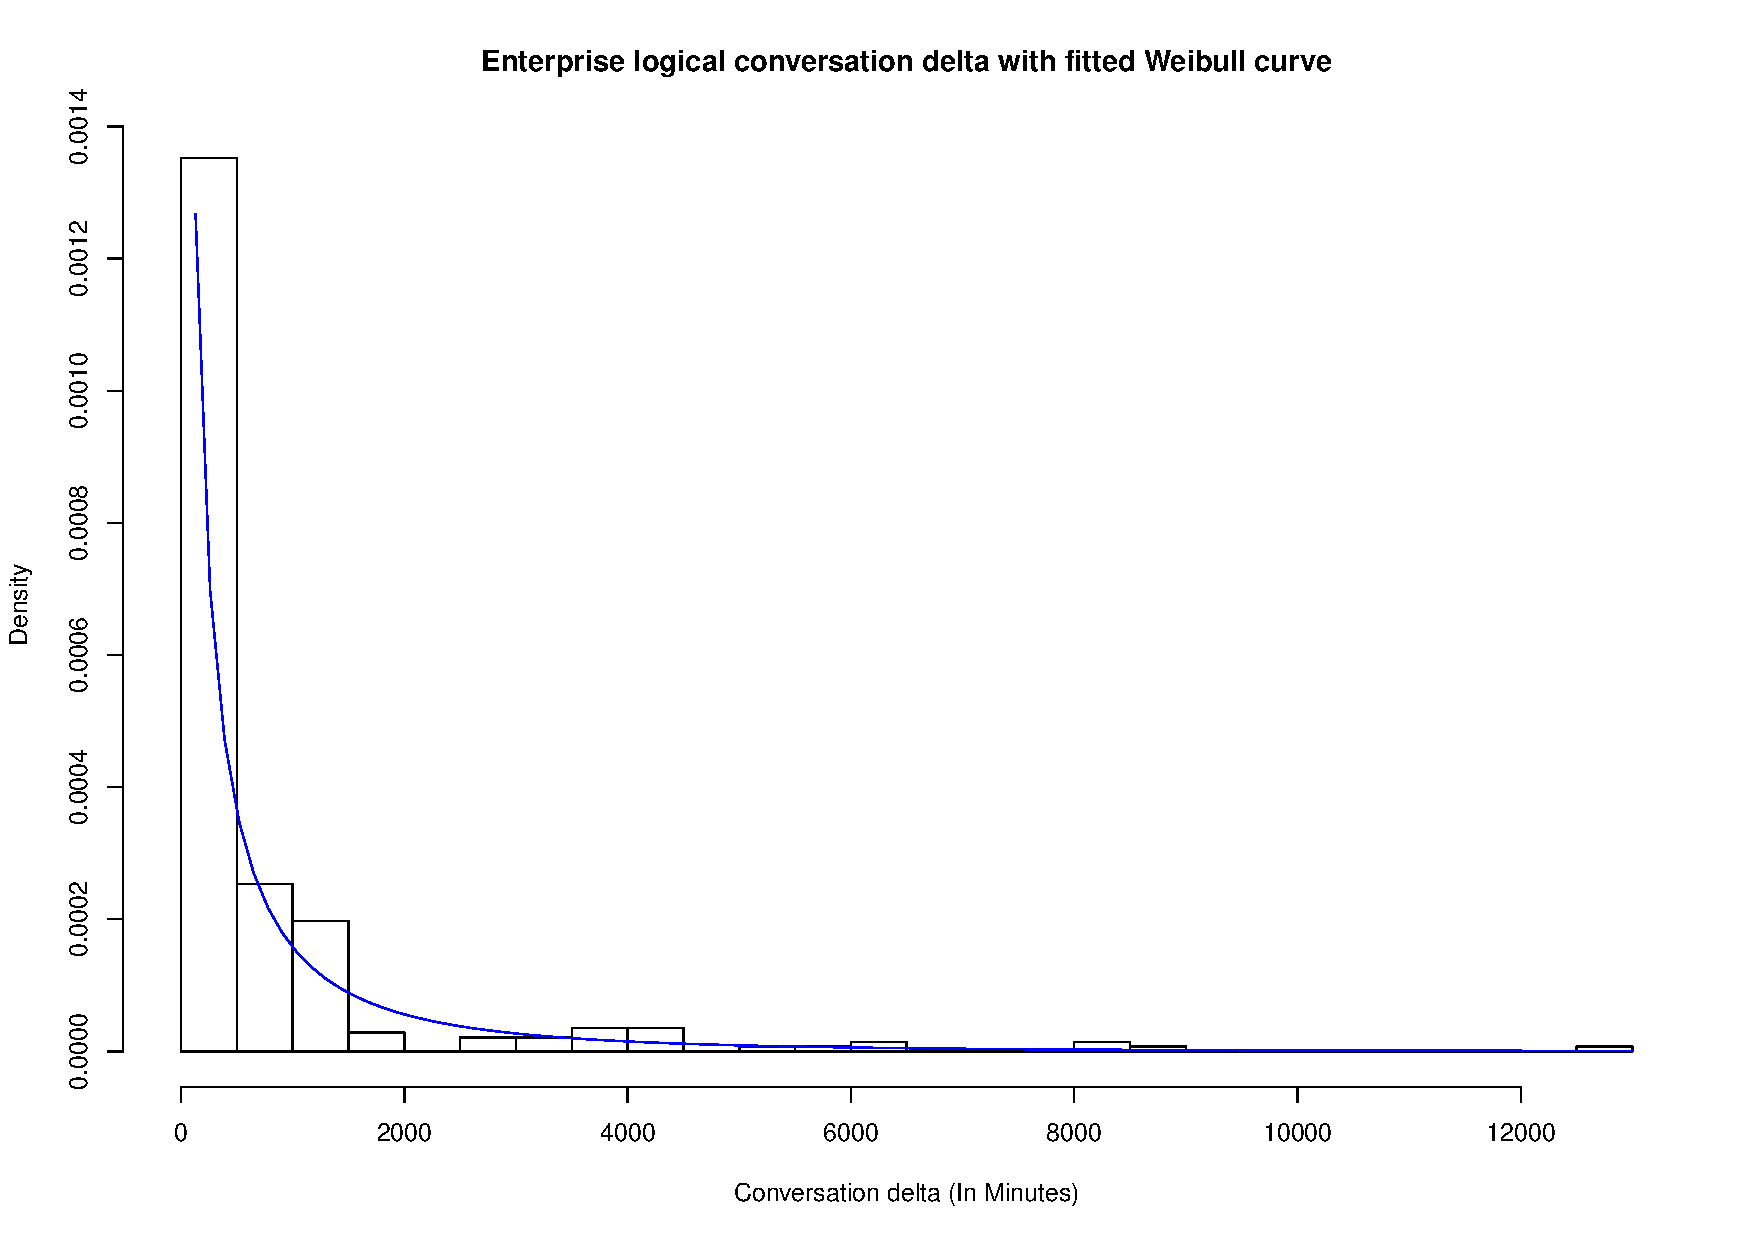
\includegraphics[height=9cm, width=8.5cm]{03_delta_logical_enterprise.pdf} 
\caption{Enterprise logical conversation delta, with fitted Weibull curve}
\end{center}
\label{fig:delta_log_ent}
\end{figure}

\begin{figure}
\begin{center}
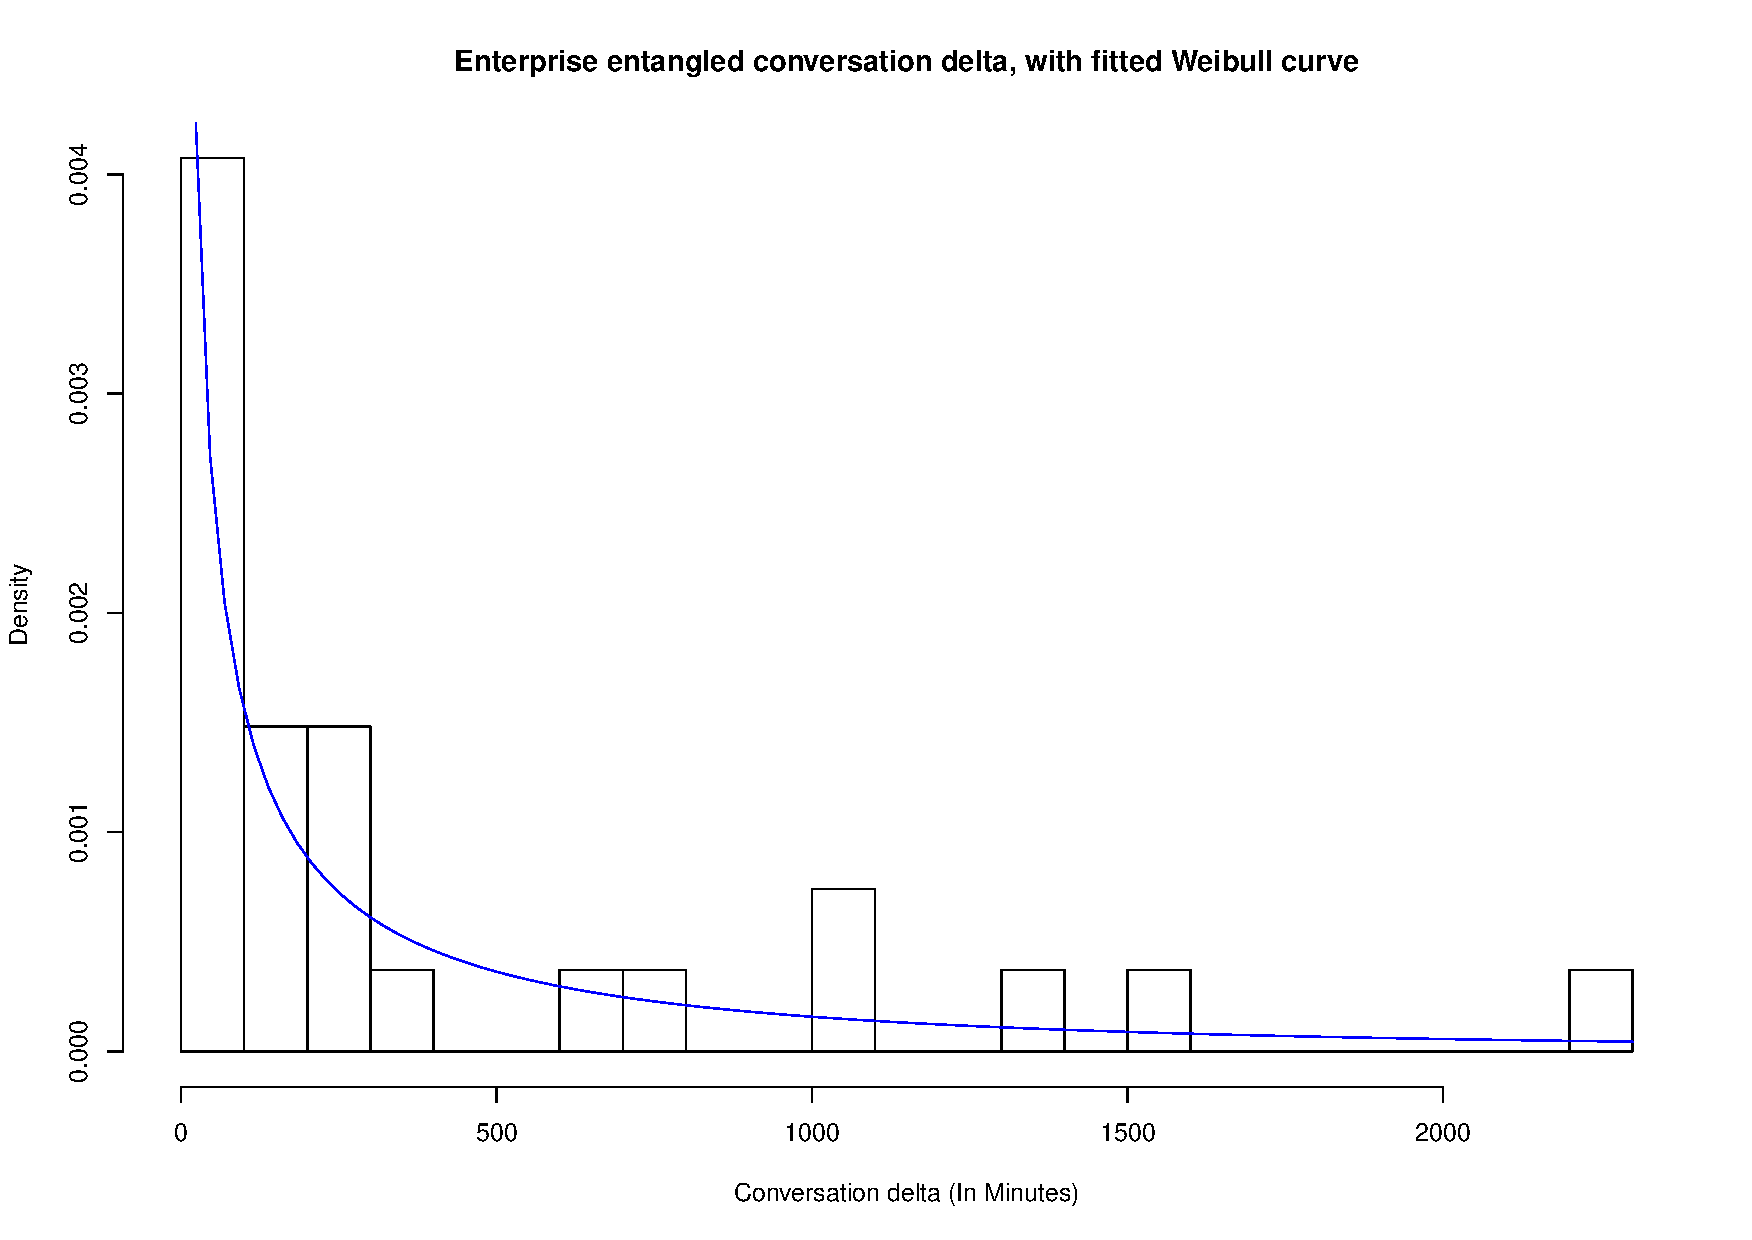
\includegraphics[height=8.5cm, width=9cm]{04_delta_entangled_enterprise.pdf} 
\caption{Enterprise entangled conversation delta with fitted Weibull curve}
\end{center}
\label{fig:delta_ent_ent}
\end{figure}

Fig. 5 shows the output of a histogram of the combined entangled and logical conversation delta times for the enterprise data set. The Sheather--Jones direct plugin bandwidth selector combined with a uniform (rectangular) shaped kernel was found to be the optimal fit.  The bandwidth was computed as 56.73.

\begin{figure}
\begin{center}
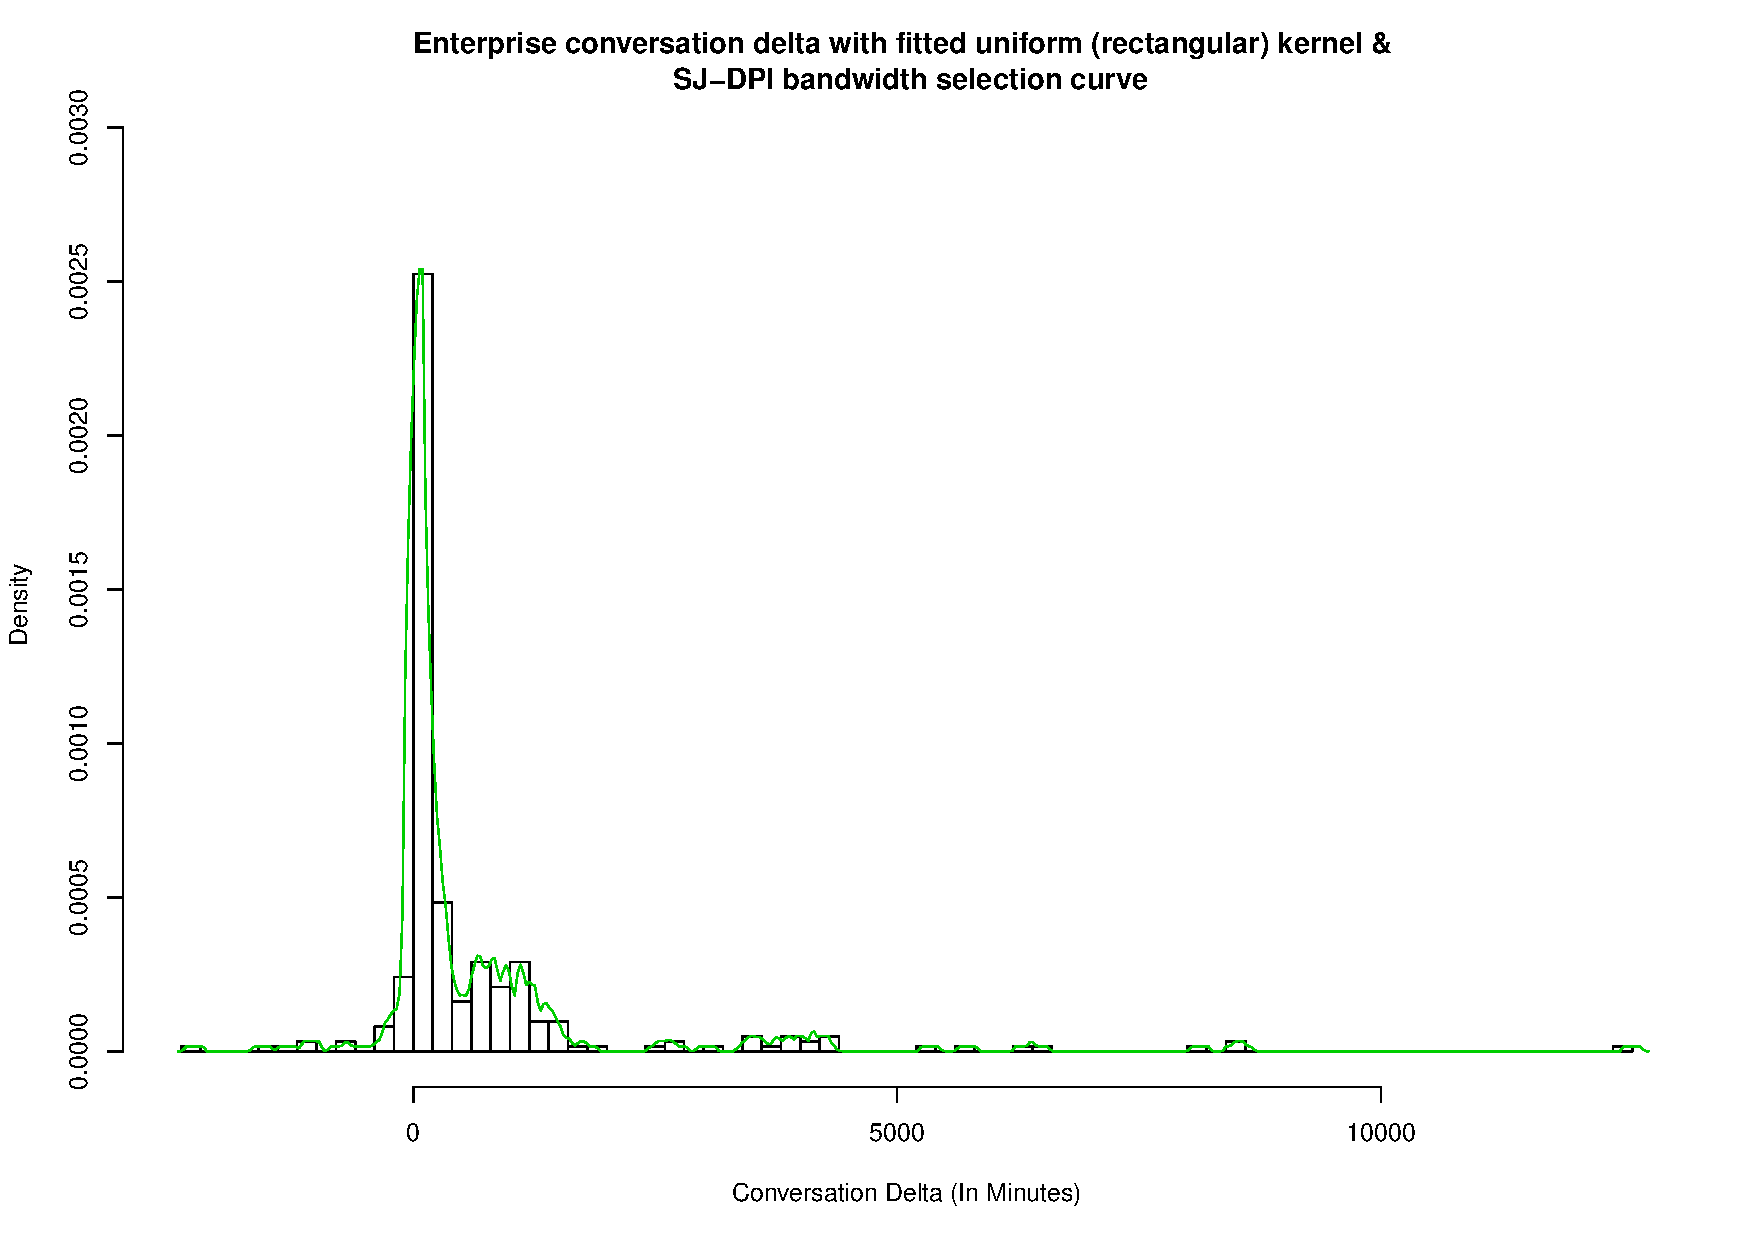
\includegraphics[height=8.5cm, width=9cm]{05_delta_kde_enterprise.pdf} 
\caption{Enterprise conversation delta with fitted uniform (rectangular) kernel & \n SJ-DPI bandwidth selection curve}
\end{center}
\label{fig:delta_kde_ent}
\end{figure}

Fig. 6 and Fig. 7 show probability density function histograms of both the entangled and logical conversation delta times for the Ubuntu dataset. A small transformation (1 minute) was added to the logical delta subset. A loglogistic distribution was found to be the best fit for both subsets.  An Anderson--Darling test statistic and p-value were computed for both distributions as 2.46 \& 0.052 (logical dataset) and 0.60 \&  0.64 (entangled dataset). In both cases the p-value was found to be above the 0.05 significance interval. For the logical dataset we quote the p-value in this case to three decimal places to illustrate the p-value was calculated as above 0.05.

\begin{figure}
\begin{center}
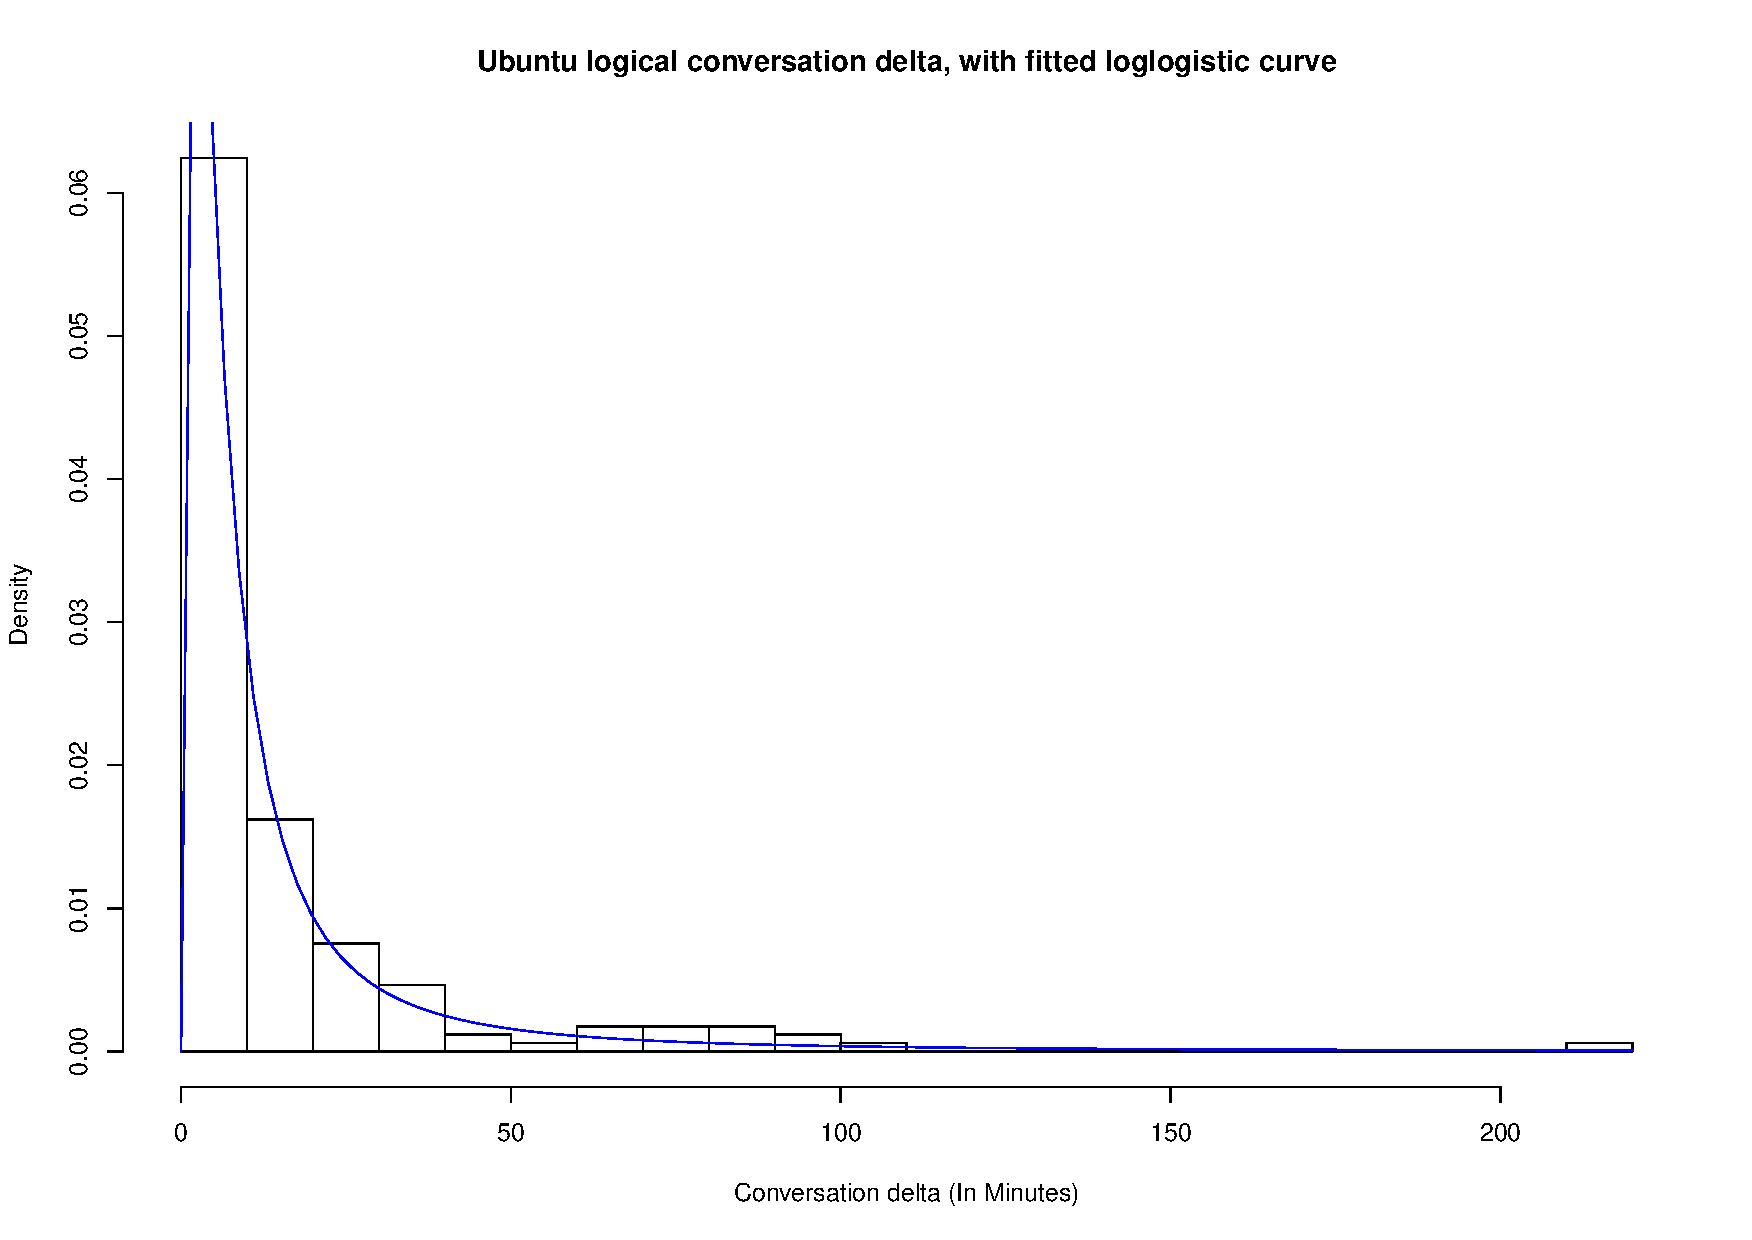
\includegraphics[height=8.5cm, width=9cm]{06_delta_logical_ubuntu.pdf} 
\caption{Enterprise logical conversation delta, with fitted Weibull curve}
\end{center}
\label{fig:delta_log_ubun}
\end{figure}

\begin{figure}
\begin{center}
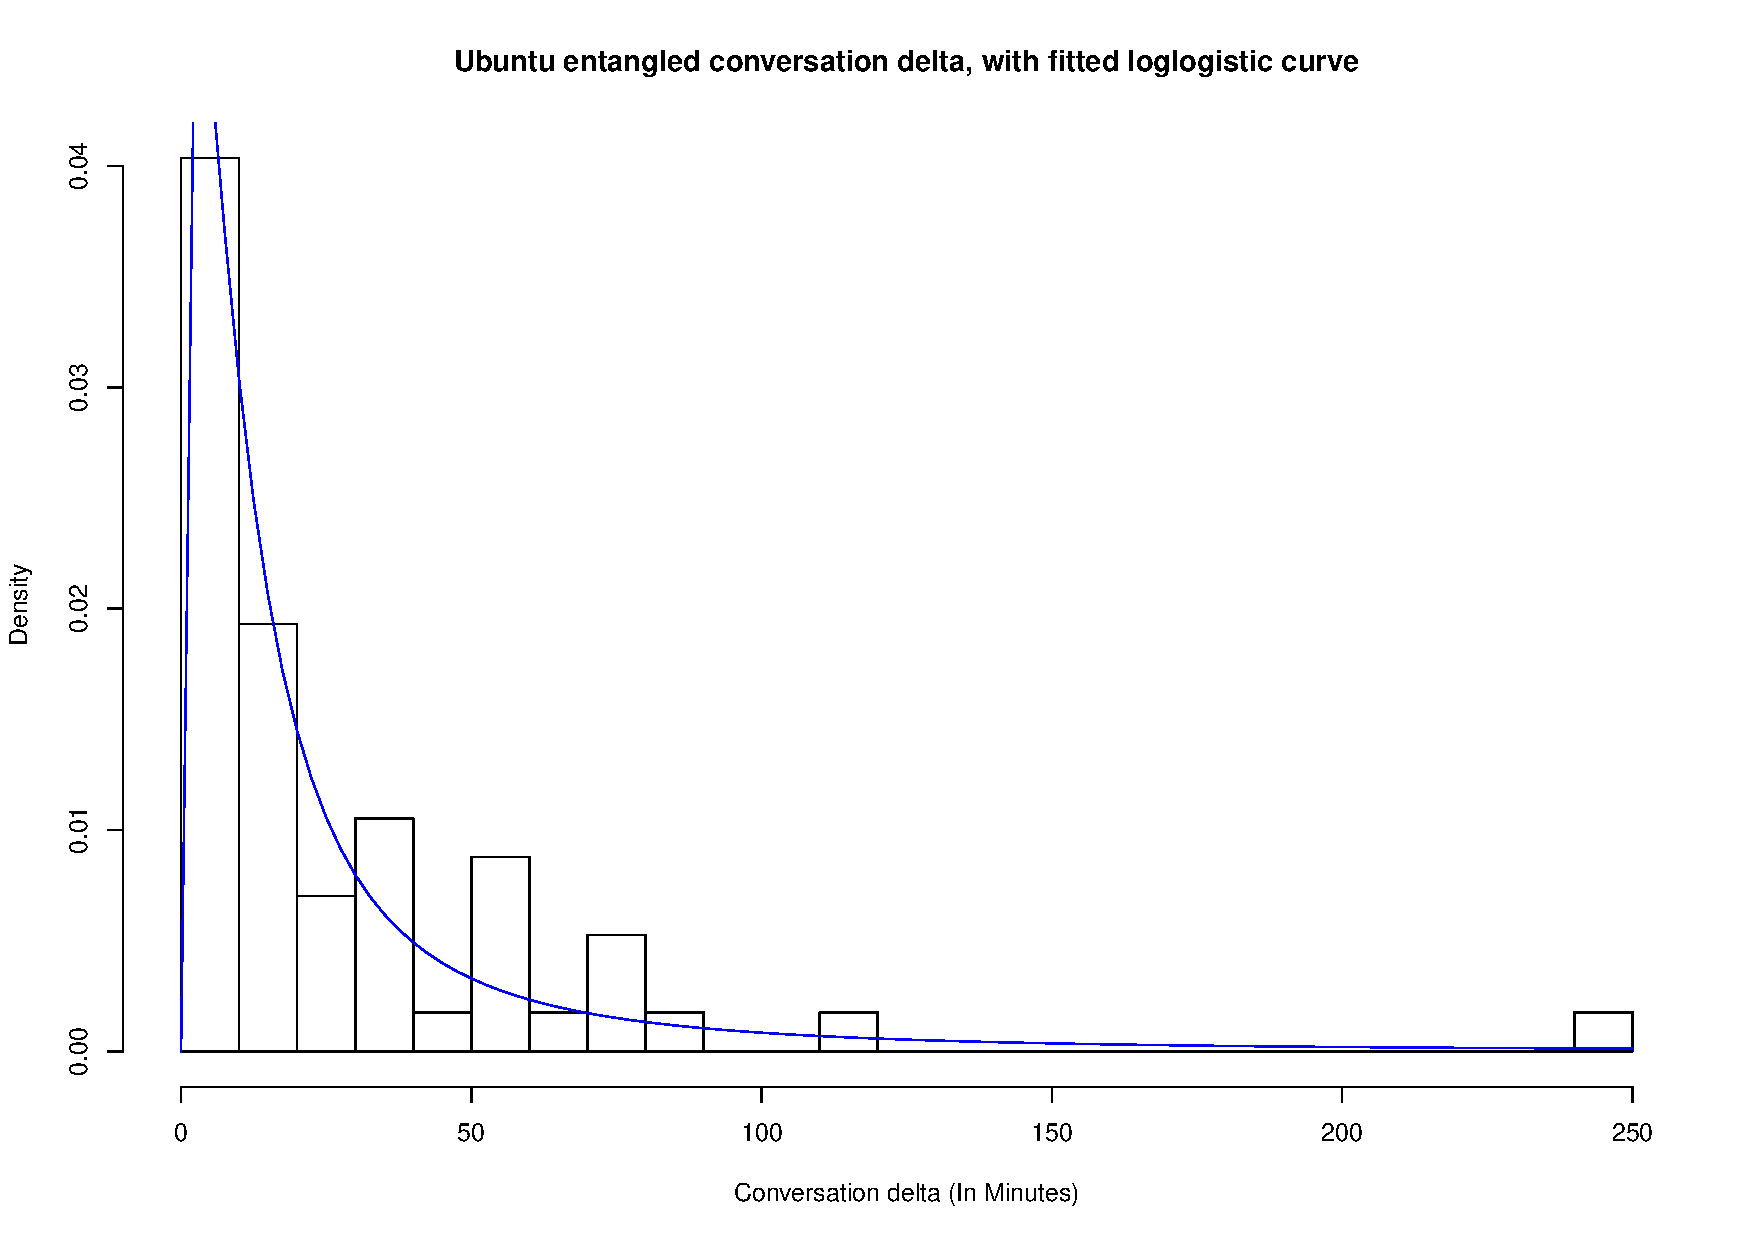
\includegraphics[height=8.5cm, width=9cm]{07_delta_entangled_ubuntu.pdf} 
\caption{Enterprise entangled conversation delta with fitted Weibull curve}
\end{center}
\label{fig:delta_ent_ubun}
\end{figure}

Fig. 8 shows the output of a histogram of the combined entangled and logical conversation delta times for the Ubuntu data set. Silverman's rule-of-thumb bandwidth selector combined with a Gaussian shaped kernel was found to be the best fit.  The bandwidth was computed as 2.94.

\begin{figure}
\begin{center}
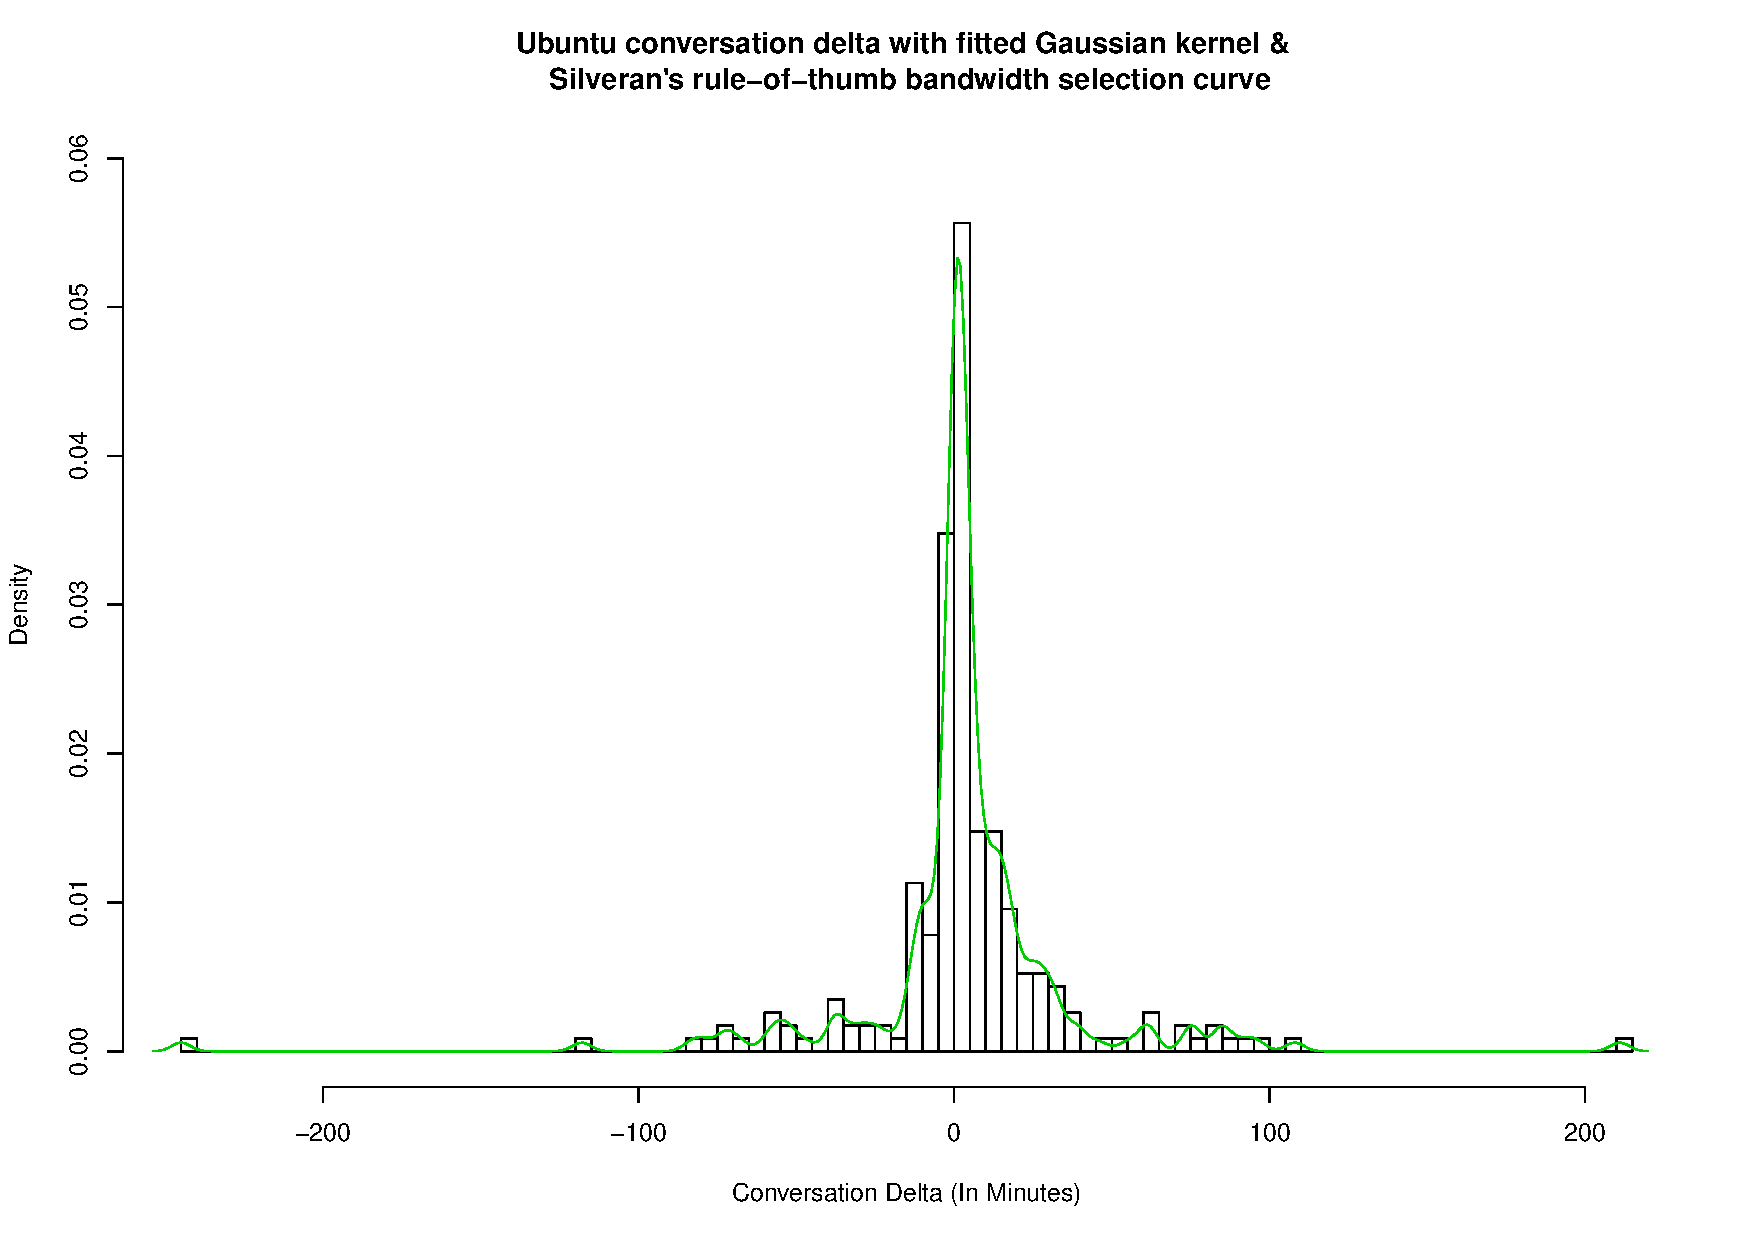
\includegraphics[height=8.5cm, width=9cm]{08_delta_kde_ubuntu.pdf} 
\caption{Enterprise conversation delta with fitted uniform (rectangular) kernel & \n SJ-DPI bandwidth selection curve}
\end{center}
\label{fig:delta_kde_ubun}
\end{figure}

\subsection{Conversation inter-arrival time modelling}


Fig. 9 shows a probability density function histogram for the enterprise dataset. A  Weibull distribution was found to be best fit. An Anderson--Darling test statistic and p-value were computed as 0.78 \& 0.5 respectively. The p-value is above the 0.05 significance interval. 

\begin{figure}
\begin{center}
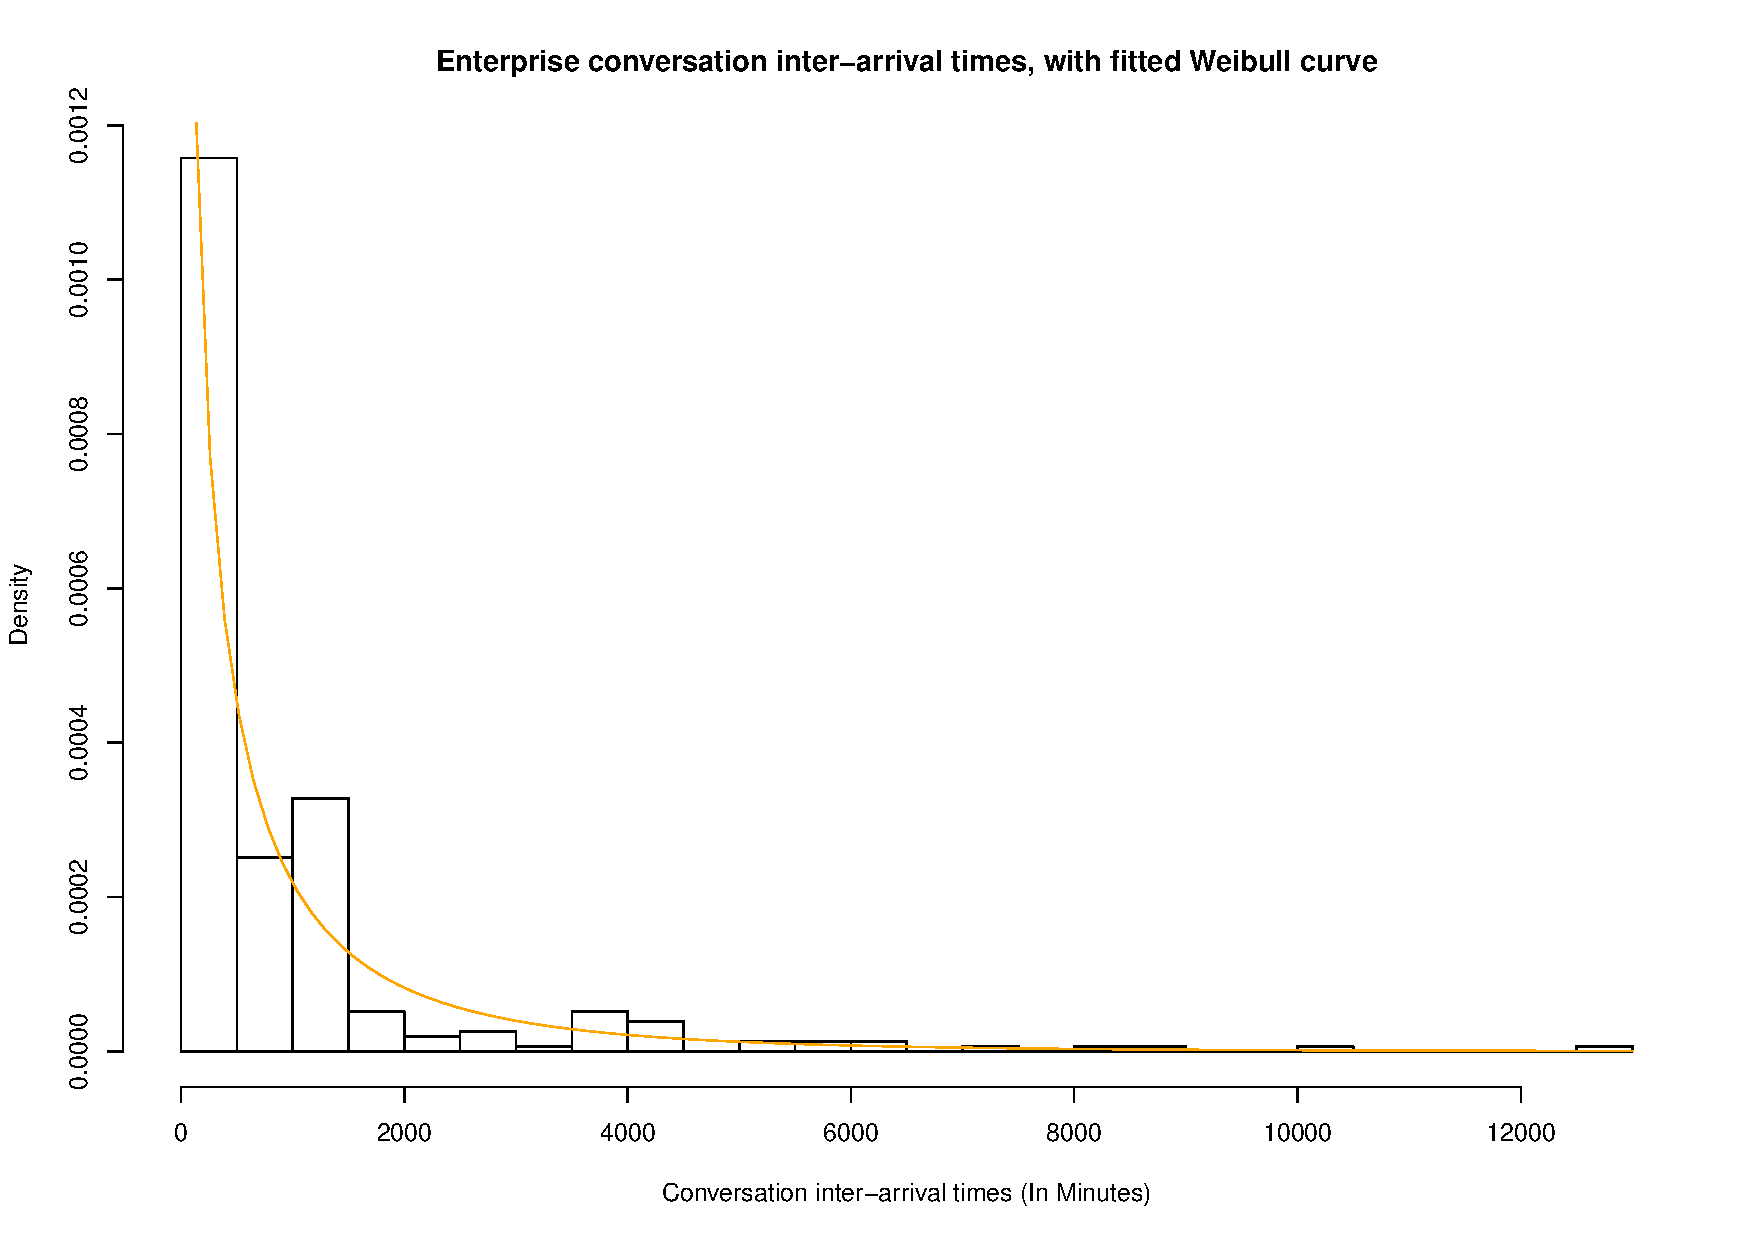
\includegraphics[height=8.5cm, width=9cm]{09_interarrival_enterprise.pdf} 
\caption{Enterprise conversation inter-arrival times with fitted Weibull curve}
\end{center}
\label{fig:interarrival_ent}
\end{figure}


Fig. 10 illustrates a probability density function histogram for the enterprise dataset. A small constant (1 minute) was applied to each value in the dataset. A loglogistic distribution was found to be best fit. An Anderson--Darling test statistic and p-value were computed as 0.72 \& 0.54 respectively. The p-value is above the 0.05 significance interval. 

\begin{figure}
\begin{center}
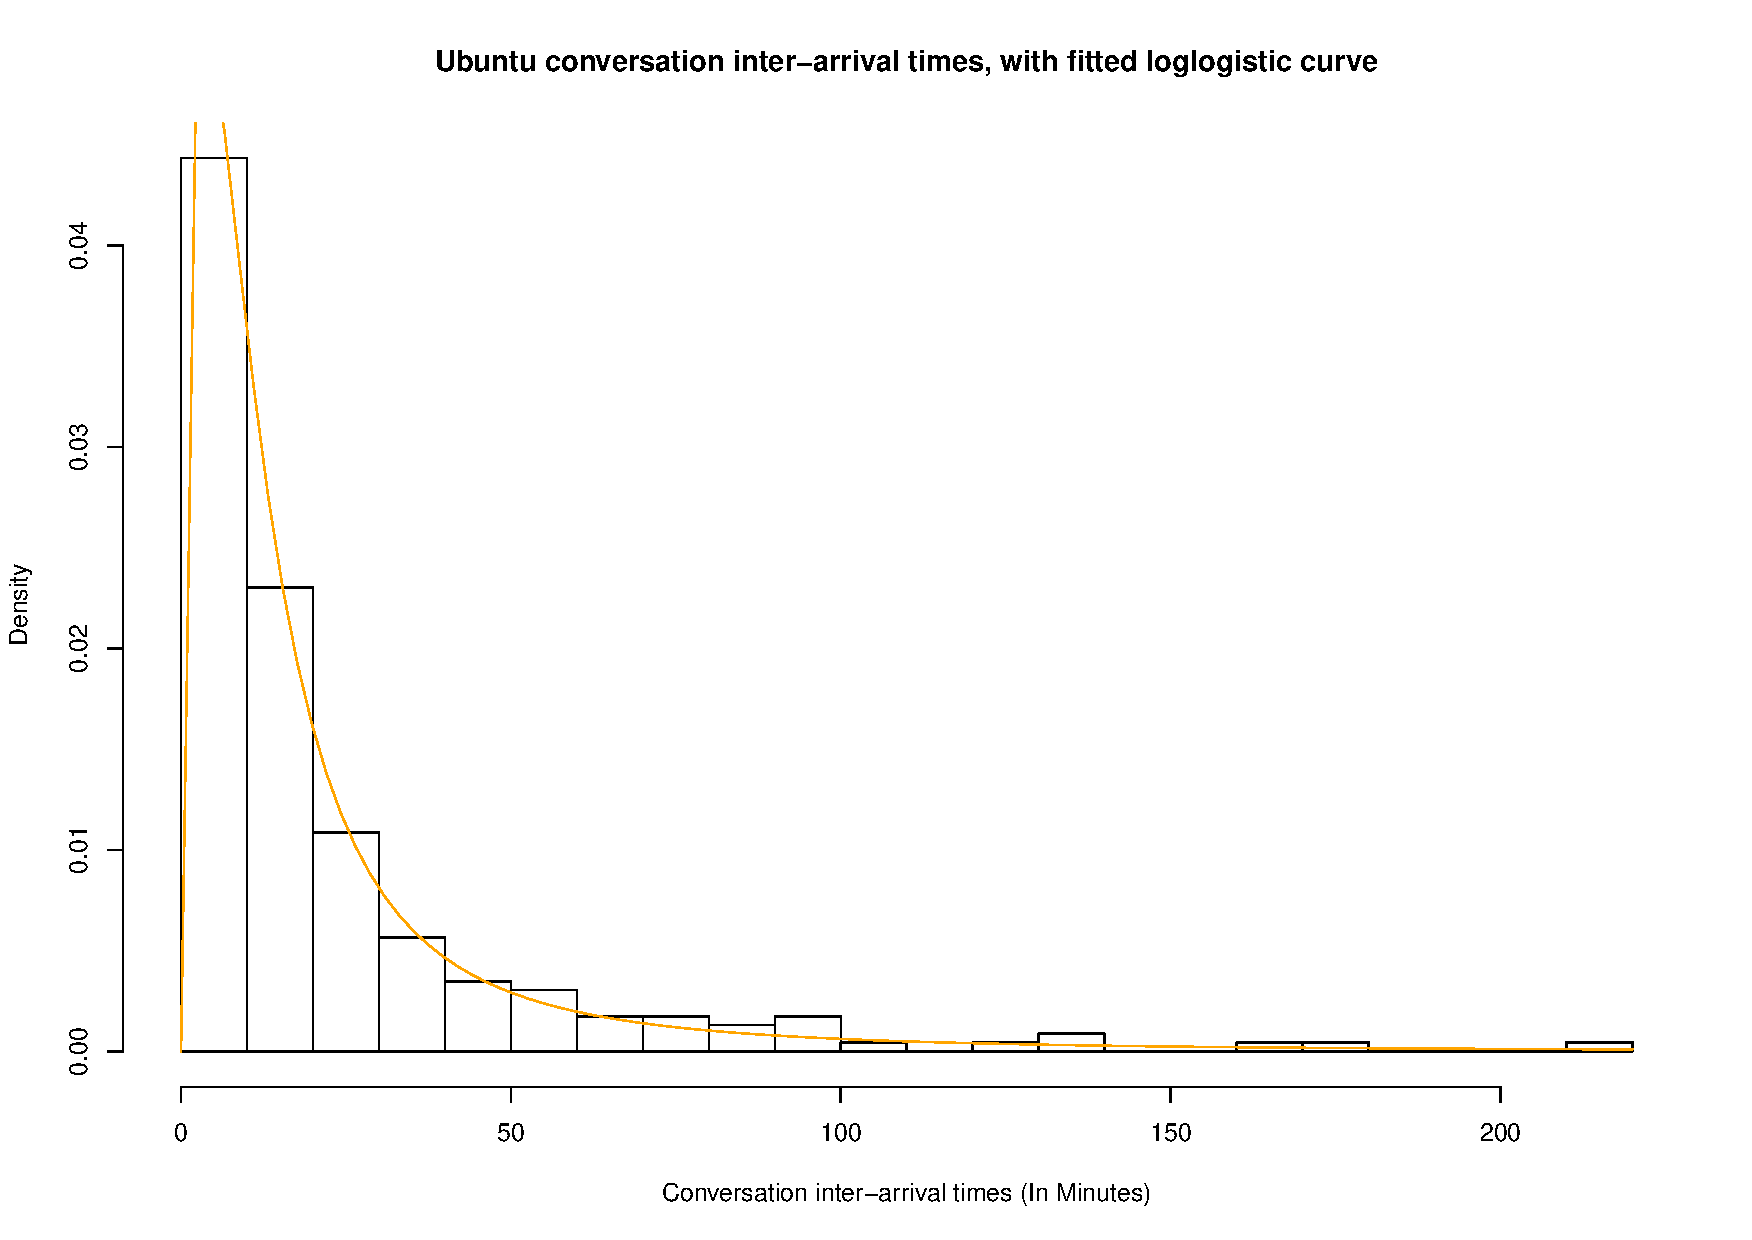
\includegraphics[height=8.5cm, width=9cm]{10_interarrival_ubuntu.pdf} 
\caption{Ubuntu conversation inter-arrival times with fitted loglogistic curve}
\end{center}
\label{fig:interarrival_ubun}
\end{figure}

\subsection{Conversation messages \& word modelling}

Fig. 11 and Fig. 12 show probability density function histograms of both the messages and words per conversation for the enterprise dataset. 
 A Burr distribution was found to be the best fit for messages per conversation. A loglogistic distribution was determined to be the best fit for words per conversation.  An Anderson--Darling test statistic and p-value was computed for both distributions as 2.13 \& 0.08 (messages per conversation dataset) and 0.65 \& 0.6 (words per conversation dataset). In both cases the p-value was found to be above the 0.05 significance interval.

\begin{figure}
\begin{center}
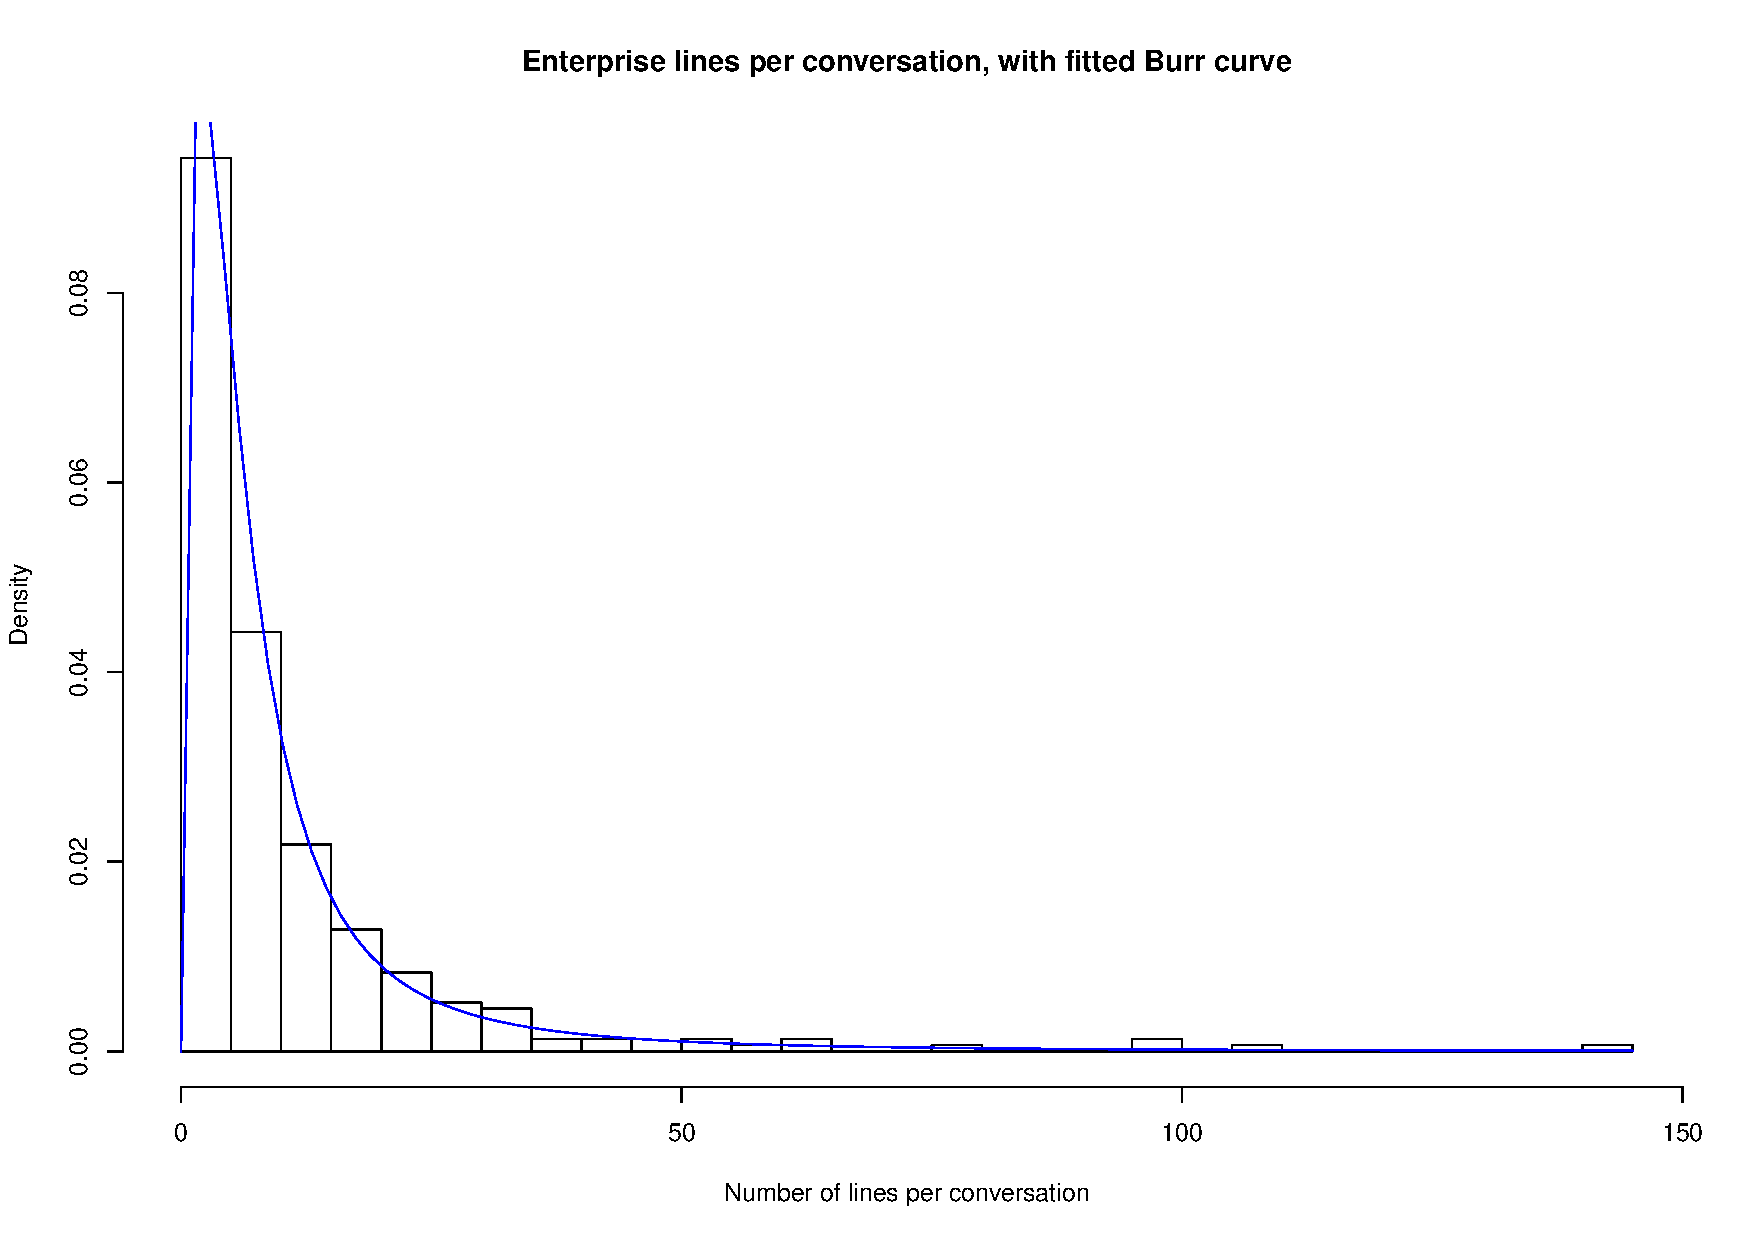
\includegraphics[height=8.5cm, width=9cm]{11_messages_enterprise.pdf} 
\caption{Enterprise messages per conversation with fitted Burr curve}
\end{center}
\label{fig:interarrival_ent}
\end{figure}

\begin{figure}
\begin{center}
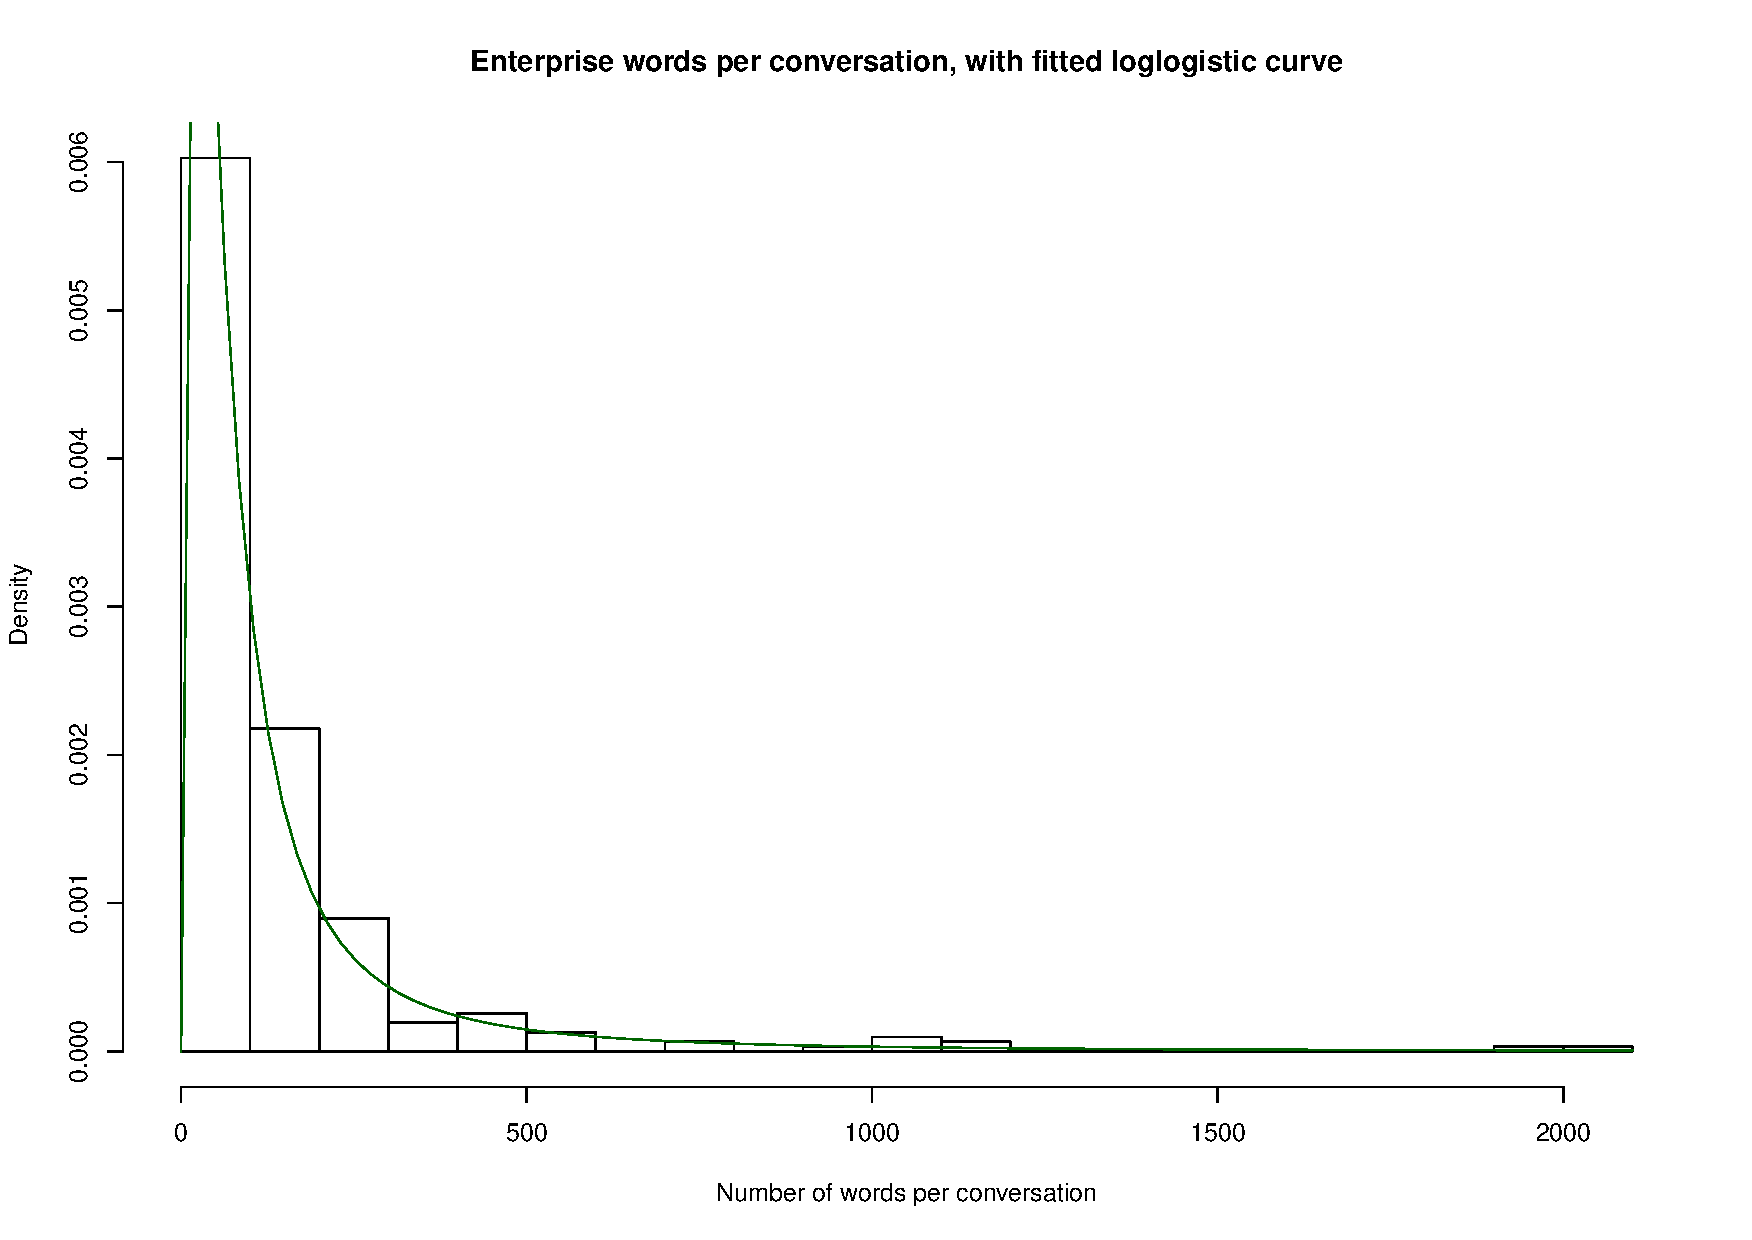
\includegraphics[height=8.5cm, width=9cm]{12_words_enterprise.pdf} 
\caption{Enterprise words per conversation with fitted loglogistic curve}
\end{center}
\label{fig:interarrival_ent}
\end{figure}

Fig. 13 and Fig. 14 show probability density function histograms of both the messages and words per conversation for the Ubuntu dataset. 
For both datasets, a Burr distribution was found to be the best fit. An Anderson--Darling test statistic and p-value was computed for both distributions as 1.76 \& 0.13 (messages per conversation dataset) and 0.19 \&  0.99 (words per conversation dataset). In both cases the p-value was found to be above the 0.05 significance interval.

\begin{figure}
\begin{center}
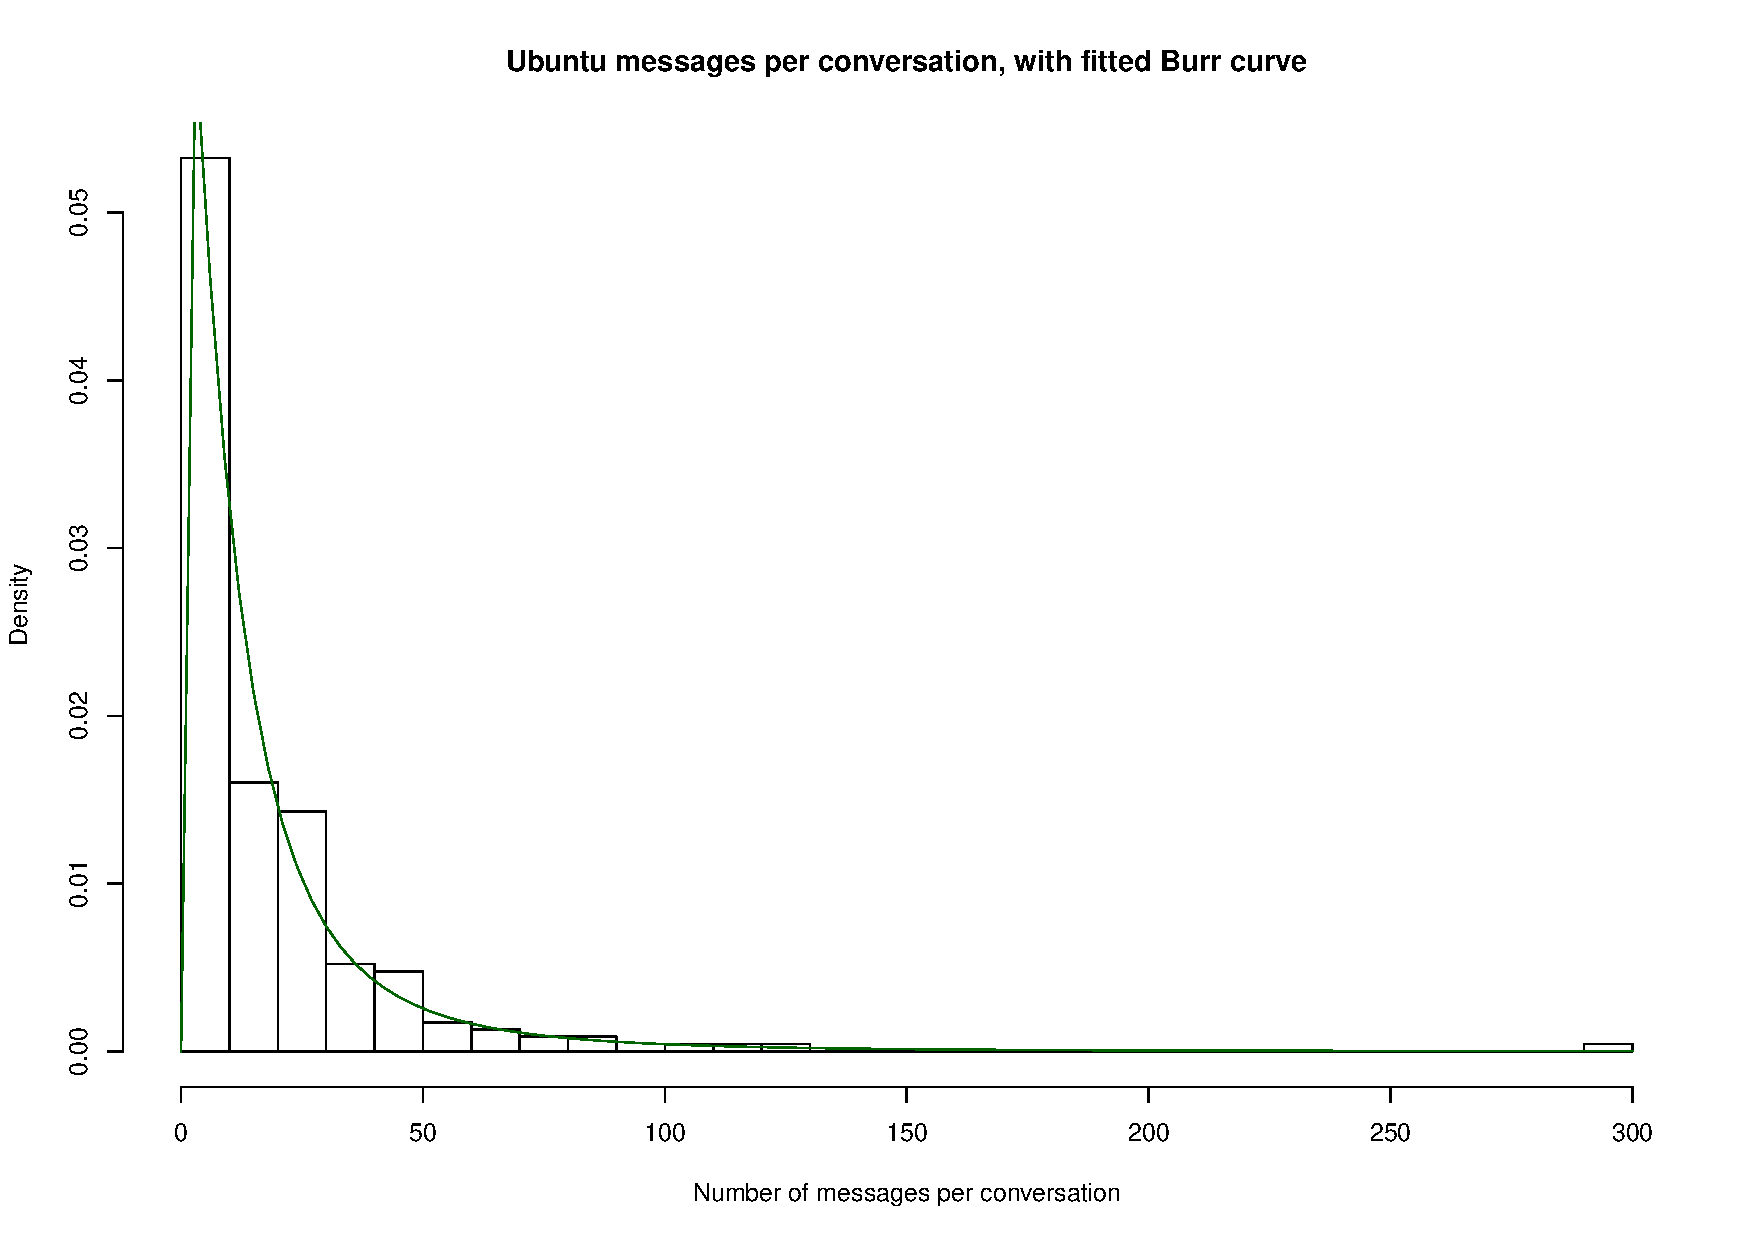
\includegraphics[height=8.5cm, width=9cm]{13_messages_ubuntu.pdf} 
\caption{Ubuntu messages per conversation with fitted Burr curve}
\end{center}
\label{fig:interarrival_ubun}
\end{figure}

\begin{figure}
\begin{center}
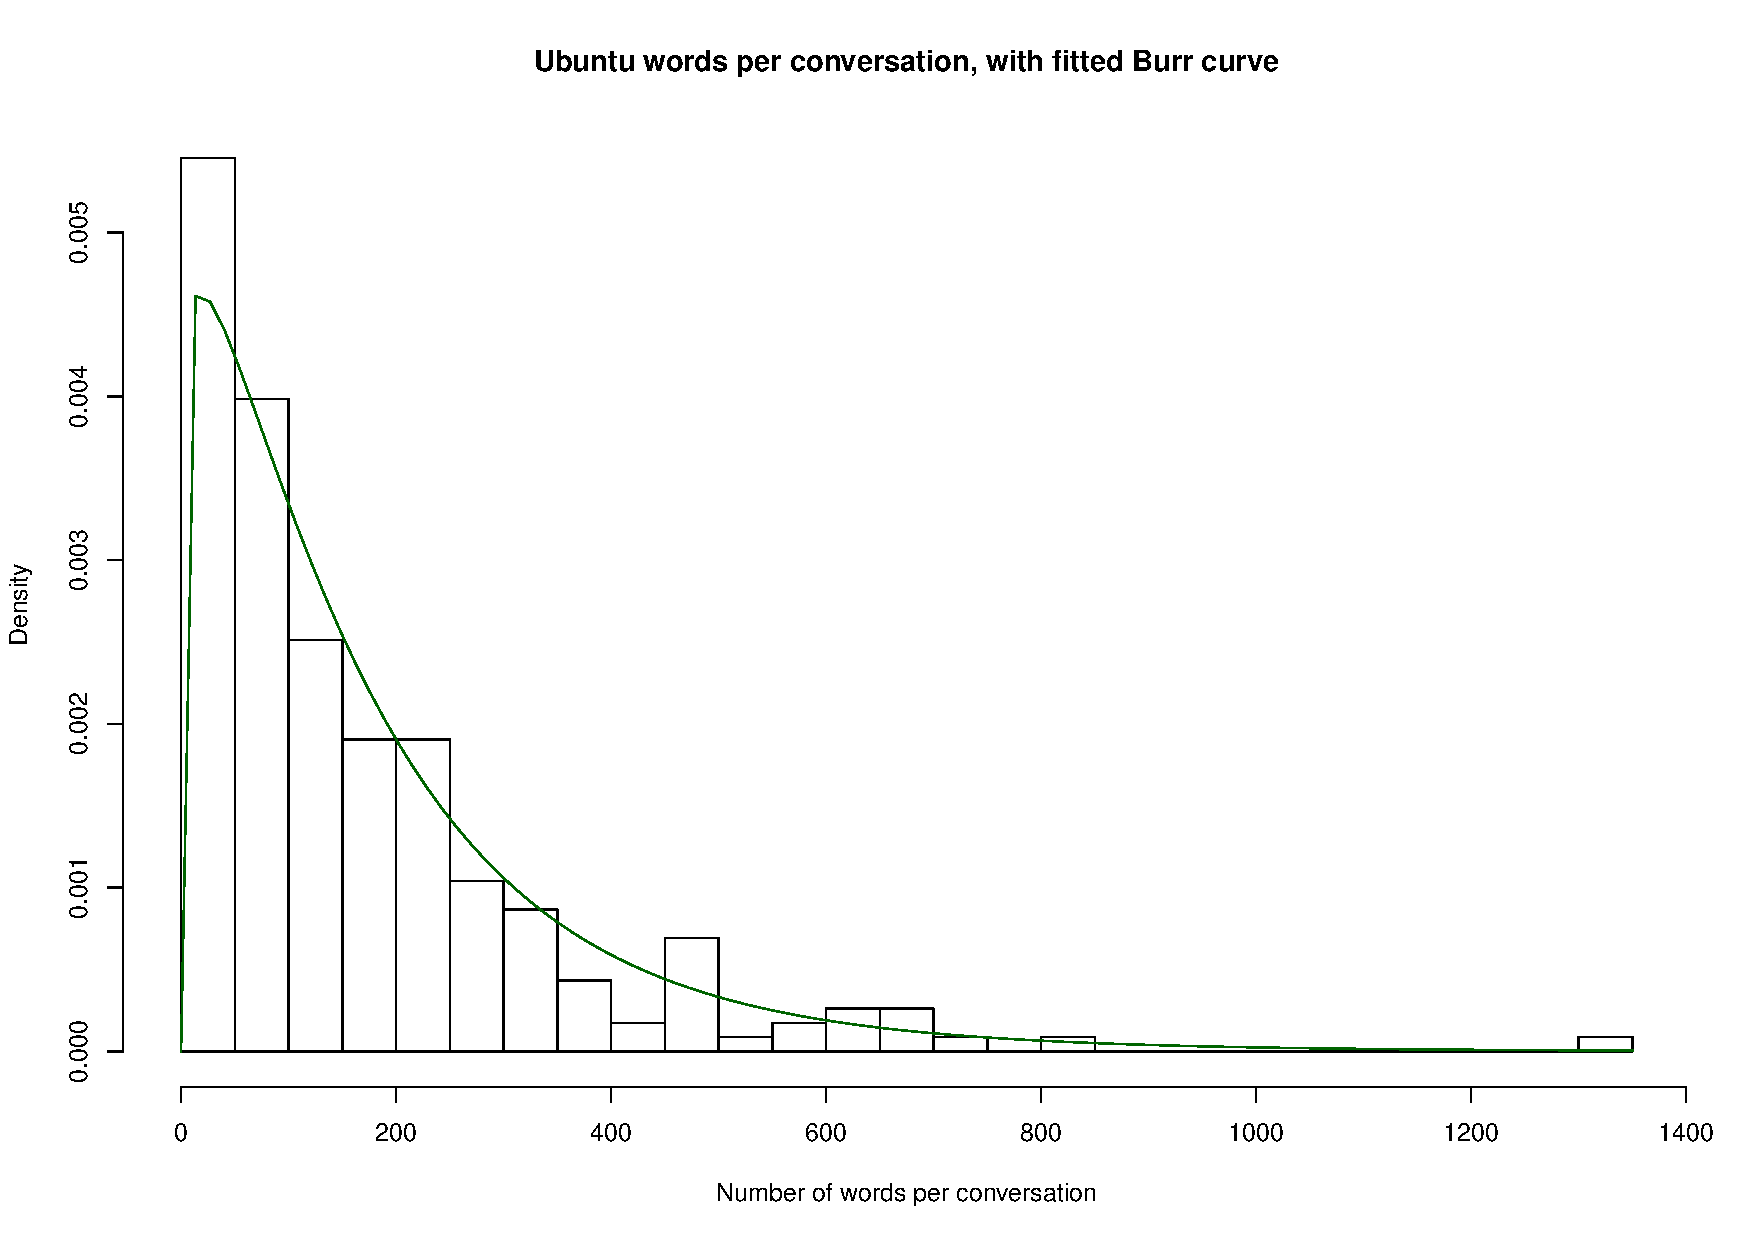
\includegraphics[height=8.5cm, width=9cm]{14_words_ubuntu.pdf} 
\caption{Ubuntu words per conversation with fitted Burr curve}
\end{center}
\label{fig:interarrival_ubun}
\end{figure}


\subsection{Conversation user count modelling}

Fig 15 illustrates the probability density function (PDF) and cumulative density function (CDF) plots of user counts per conversation for the enterprise dataset. However using the raw counts a Poisson distribution was found to be a poor fit due to an under-dispersion within the dataset. A hurdle method was implemented whereby the counts of n-1 users were modelled. A chi-squared test statistic, degrees of freedom and p-value were calculated with the hurdle method applied. The values computed were 2.97, 4 and 0.56 respectively. It was noted the p-value was above the 0.05 significance.


\begin{figure}
\begin{center}
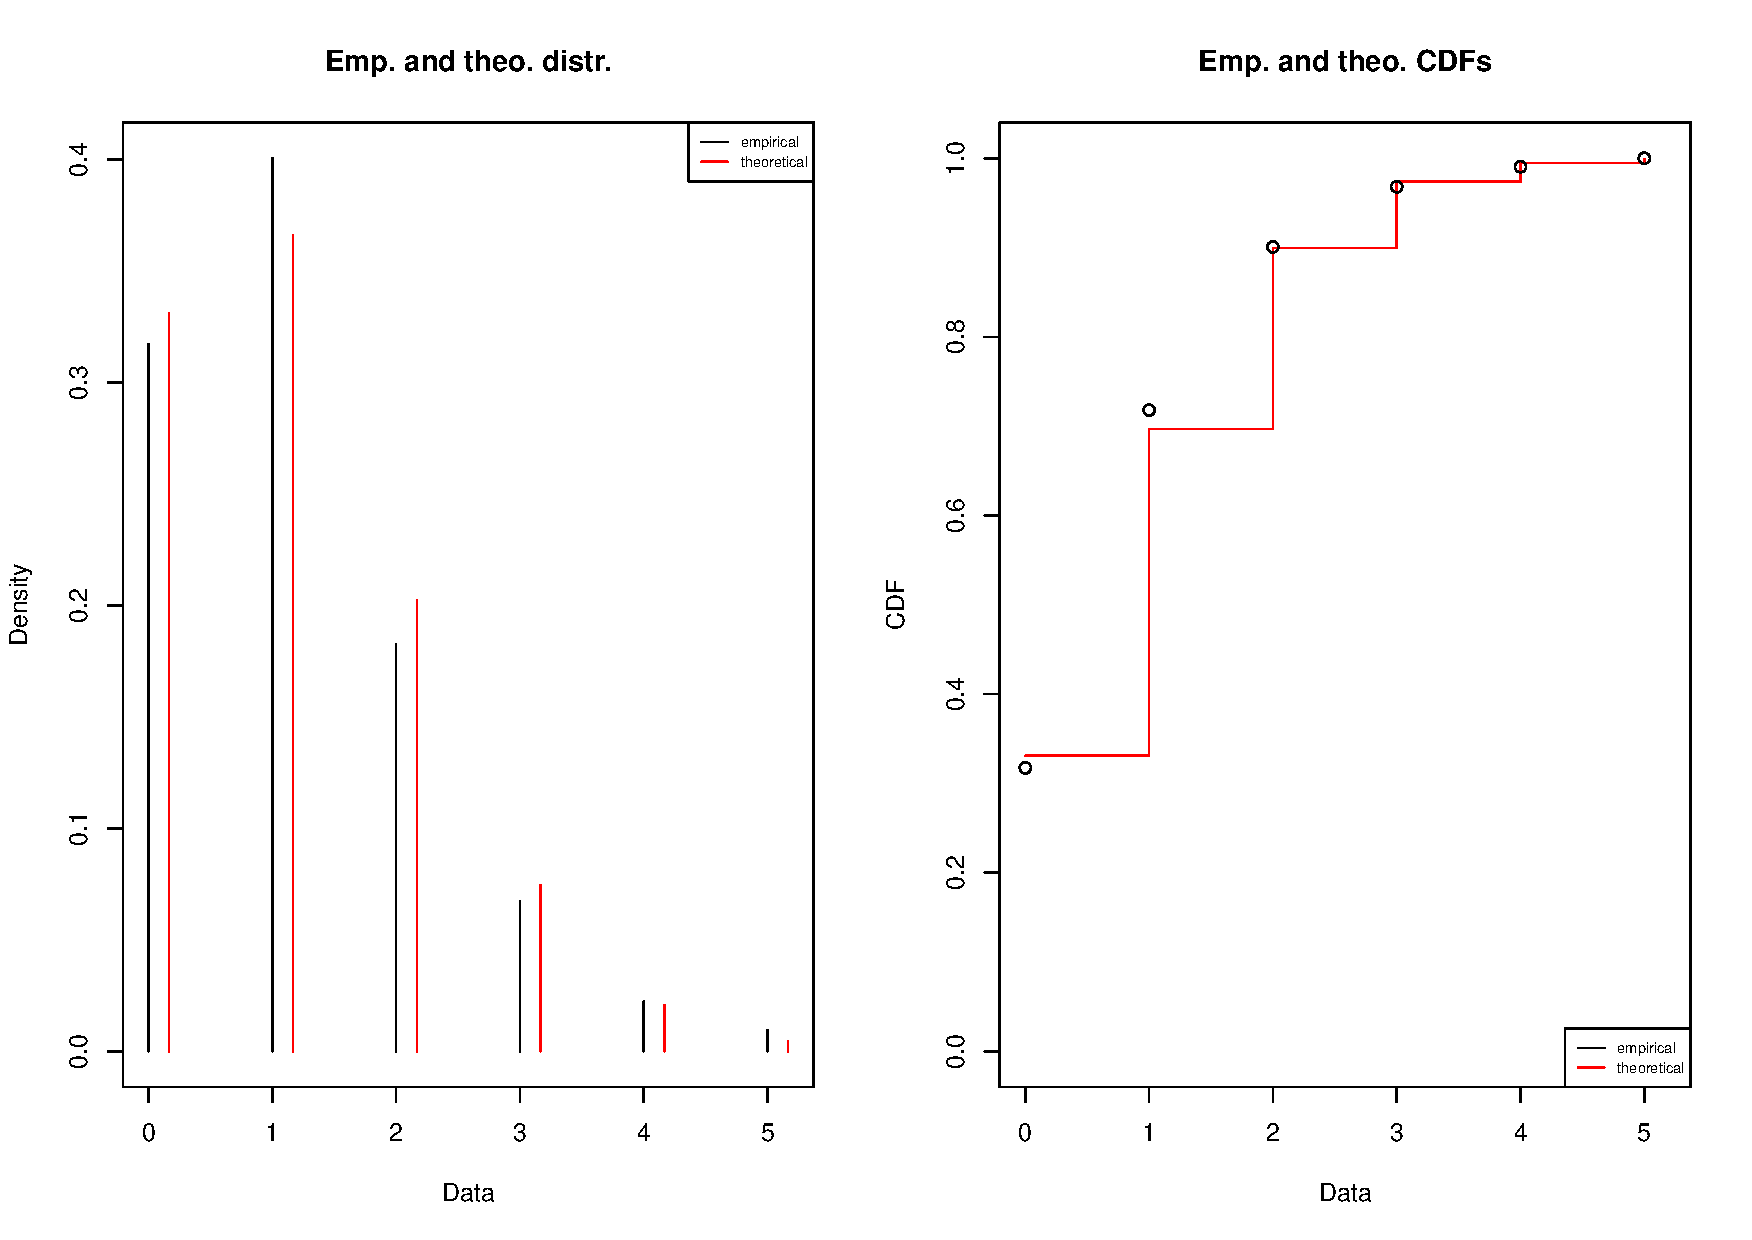
\includegraphics[height=8.5cm, width=9cm]{15_users_enterprise.pdf} 
\caption{Enterprise N-1 users per conversation with fitted Poisson PDF and CDF}
\end{center}
\label{fig:interarrival_ent}
\end{figure}

Fig 16 illustrates the PDF and cumulative density function CDF  plots of user counts per conversation for the enterprise dataset. However using the raw counts a Poisson distribution was found to be a poor fit. A similar hurdle method was applied to the count data as described for the enterprise data set. A chi-squared test statistic, degrees of freedom and p-value were calculated with the hurdle method applied. The values computed were 11.08, 5 and 0.05 respectively. It was noted the p-value was exactly 0.05 and not above the 0.05 significance.



\begin{figure}
\begin{center}
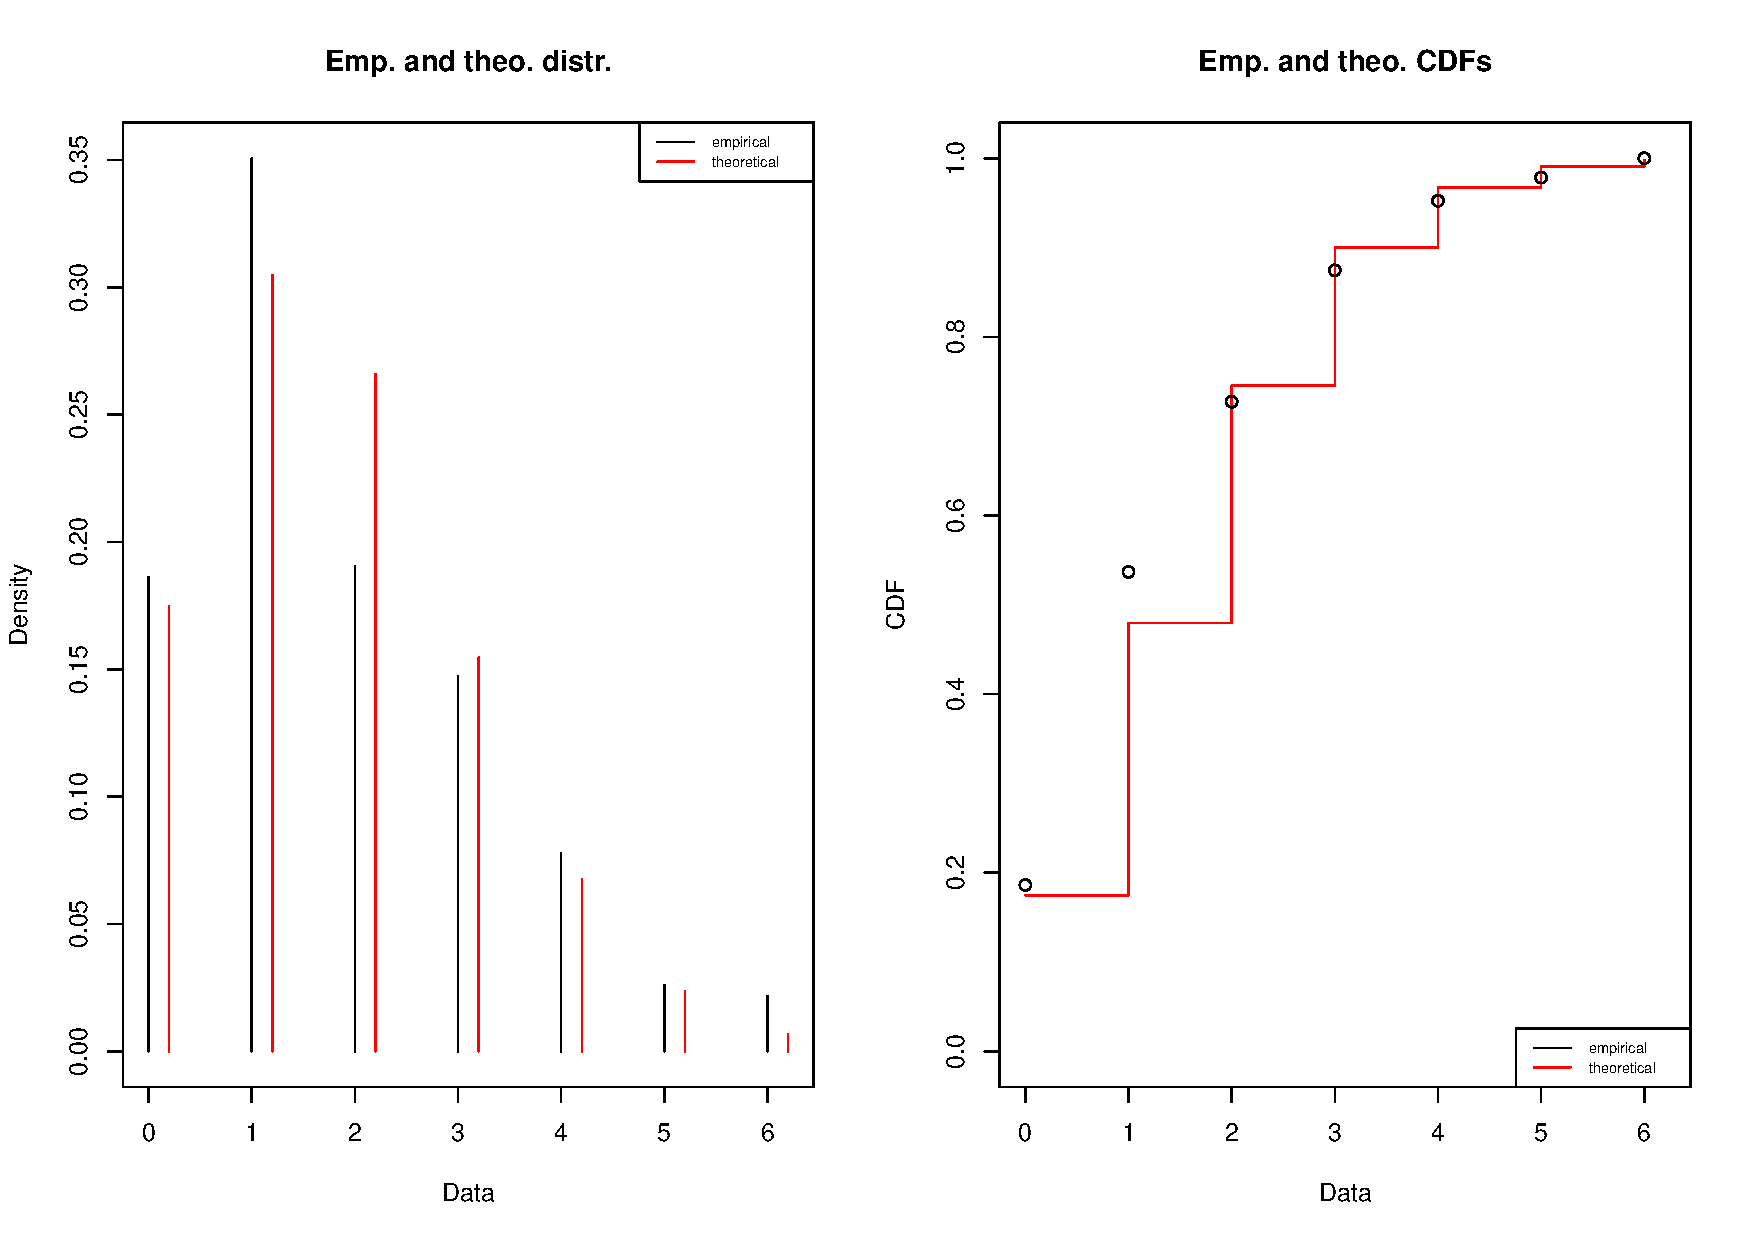
\includegraphics[height=8.5cm, width=9cm]{16_users_ubuntu.pdf} 
\caption{Ubuntu N-1 users per conversation with fitted Poisson PDF and CDF}
\end{center}
\label{fig:interarrival_ent}
\end{figure}

\section{Discussion}

Section IV provided a summary of modelling experiments that were conducted as part of his study. The following section provides deeper analysis and discussion of the results. In each section references will be made to each research question asked in section III.

Prior to a detailed discussion of our results, we summarise the results along with each corresponding research question. Table~\ref{tab:researchsummary} provides this summary.

\begin {table*}[]
\caption {Summary of research question, results and techniques used}
\label{tab:researchsummary}
\begin{flushleft}
\begin{tabular}{| p{1cm} | p{4.6cm} | p{5.4cm} | p{5.4cm} |} \hline \bf{Dataset} & \bf{Research Question} & \bf{Results} & \bf{Data Transformation \& Fitting techniques} 
\\ \hline Enterprise & 1. What method can be used to model conversation duration times? & Weibull distribution is the best fit. \par AD test statistic = 1.30 \par p-value = 0.23 & Zero values removed using Hurdle method. \cite {mullahy1986specification} \par MLE \cite{fisher1925theory} \cite {wilks1938large}

\\ \hline Ubuntu & 1. What method can be used to model conversation duration times? & Burr / loglogistical distribution is the best fit. \par AD test statistic = 1.10 \par p-value = 0.31  & Zero values removed using Hurdle method. \cite {mullahy1986specification} \par MLE \cite{fisher1925theory} \cite {wilks1938large}


\\ \hline Enterprise & 2. What method can be used to model conversation delta times? & 
(Combined) No suitable parametric fit found. 
\par (Combined)  Uniform kernel with SJ-dpi bandwidth = 56.73
\par (Entangled)  Weibull distribution is the best fit.
\par (Entangled) AD test statistic = 0.30, p-value = 0.94
\par (Logical)  Weibull distribution is the best fit.
\par (Logical) AD test statistic = 0.94, p-value = 0.76
& 
(Combined) KDE Non-Parametric method used. \cite{rosenblatt1956remarks}\cite{parzen1962estimation}
\cite{sheather1991reliable} 
\par (Entangled) Absolute values used. MLE \cite{fisher1925theory} \cite {wilks1938large}
\par (Logical) MLE \cite{fisher1925theory} \cite {wilks1938large}

\\ \hline Ubuntu & 2. What method can be used to model conversation delta times? & 
(Combined) No suitable parametric fit found. 
\par (Combined)  Gaussian kernel with rule-of-thumb bandwidth = 2.94
\par (Entangled)  loglogistic distribution is the best fit.
\par (Entangled) AD test statistic = 0.60, p-value = 0.64
\par (Logical)  loglogistic distribution is the best fit.
\par (Logical) AD test statistic = 2.46, p-value = 0.052
& 
(Combined) KDE Non-Parametric method used. \cite{rosenblatt1956remarks}\cite{parzen1962estimation}
\cite{silverman1986density}  
\par (Entangled) Absolute values used. MLE \cite{fisher1925theory} \cite {wilks1938large}
\par (Logical) A 1 minute value was added to each delta time (x+1). MLE \cite{fisher1925theory} \cite {wilks1938large}


\\ \hline Enterprise & 3. What method can be used to model conversation inter-arrival times?  & Weibull distribution is the best fit. \par AD test statistic = 0.78 \par p-value = 0.50 & MLE \cite{fisher1925theory} \cite {wilks1938large}

\\ \hline Ubuntu & 3. What method can be used to model conversation inter-arrival times? & loglogistic distribution is the best fit. \par AD test statistic = 0.72 \par p-value = 0.54 & A 1 minute value was added to each inter-arrval time (x+1). \par MLE \cite{fisher1925theory} \cite {wilks1938large}

\\ \hline Enterprise &  4. What method can be used to model conversation message and word counts? & 
(Messages) Burr distribution is the best fit. 
\par (Messages) AD test statistic = 2.13,  p-value = 0.08 
\par (Words) loglogistic distribution is the best fit.  
\par (Words) AD test statistic = 0.65,  p-value = 0.60  &
MLE \cite{fisher1925theory} \cite {wilks1938large}

\\ \hline Ubuntu &  4. What method can be used to model conversation message and word counts? & 
(Messages) Burr distribution is the best fit. 
\par (Messages) AD test statistic = 1.76,  p-value = 0.13 
\par (Words) Burr distribution is the best fit.  
\par (Words) AD test statistic = 0.19,  p-value = 0.99  &
MLE \cite{fisher1925theory} \cite {wilks1938large}


\\ \hline Enterprise &  5. Can a Poisson distribution be used to model conversation user counts? & 
Strong evidence to suggest Poisson is a good fit. 
\par {$\chi$}^2  = 2.97
\par degrees of freedom = 4
\par p-value = 0.56 & 
User counts were reduced by 1 for all values and n-1 users were modelled and fitted. \cite {mullahy1986specification} 

\\ \hline Ubuntu &  5. Can a Poisson distribution be used to model conversation user counts? & 
Borderline evidence to suggest Poisson is a good fit. 
\par {$\chi$}^2  = 11.08
\par degrees of freedom = 5
\par p-value = 0.05 & 
User counts were reduced by 1 for all values and n-1 users were modelled and fitted. \cite {mullahy1986specification} 
\\ \hline 
 \end{tabular}
\end{flushleft}
\end{table*}

\subsection{Conversation duration modelling}

The results section has shown that a parametric approach to model conversation durations is reasonable. For the enterprise dataset the Weibull distribution was the best fit. For the Ubuntu data set either a Burr or log-logistic distribution proved to be the best fit. In both cases we remark that the p-value for the Anderson-Darling Goodness of fit was well above the 0.05 significance interval. \par

Of interest is that, in order to produce the above fit, given that conversation duration were measured in minutes by the system logs, any durations of 0 minutes were removed from the dataset. The removal of 0's from a data set is typically undertaken as part of a hurdle model technique. We feel this is a reasonable approach as we are primarily interested in modelling conversations of a positive duration. It should be noted that the percentage of conversations removed were 23\% and 17\% for the enterprise and Ubuntu data sets respectively. \par

This study as has answered our first research question: Can the duration of annotated chat conversations be modelled by a parametric method. Data analysts from micro teams and startups can use the result of this work to compute a mean and standard deviation for their modelled distribution. These measures of location can then be used to compute the expected duration of a conversation and the proportion of conversations that will last a fixed duration. If we think of conversations within a real-time messaging application as vehicle to discuss and diagnose complex problems, this result can be used as a way to model service time diagnosis and resolution. \par

Finally it should be noted that for each dataset, a different distribution result was produced. As we have noted previously the Ubuntu dataset has a greater ratio of messages per hour, it seems intuitive that a heavier tailed distribution (log-logistic) would be an appropriate fit. \par

\subsection{Conversation delta time modelling}

We have learned from our results that no suitable parametric could be found to model overall conversation delta times. As we used a method to differentiate between entangled and logical delta times, a two tailed histogram was produced. We have seen that by using a non-parametric such as KDE, a suitable bandwidth selector and kernel shape can be computed. Once again we can see the results vary depending on the dataset used. For the enterprise data set a uniform kernel with a Sheather Jones direct plugin was found to be the most appropriate method and fit. For the Ubuntu data a Gaussian kernel using Silverman's rule-of-thumb bandwidth selector yielded the best approach.

Conversely our study found that by dividing the conversation delta times into entangled and logical delta subsets, a parametric method can be used for data modelling. Initiatively we found that Weibull and log-logistic distributions were the most appropriating fitting distributions. We remark, that these distributions are the same as the ones used to model conversation duration. In all cases they p-value of each fit exceeded the 0.05 significance interval. However we note that for modelling of logical delta times from the Ubuntu data set, our p-value was computed to three decimal places to ensure the p-value was greater than the significance interval. This specific result should be treated with some caution.

This piece of research has answered our second research question. Clearly for datasets with entangled and logical delta times, a non-parametric approach is our preferred option. However if a parametric approach is required, by subsetting the data, a result (showing an appropriate distribution may be possible). If we think of the conversation delta times as the downtime between conversations, location measures can be computed. These measures can then be used to forecast the downtimes of team discussion in a collaborative environment.

\subsection{Conversation inter-arrival time modelling}

For our third research question we asked what is the most appropriate method to model conversation inter-arrival times. We learned that once again the Weibull and log-logistic distributions were the most appropriate fits for the enterprise and Ubuntu datasets respectively. We know that the inter-arrival time is a function of conversation duration and delta times. Therefore it's intuitive that same type of distribution was found to model a time period which spans both the duration and delta times. For both data sets we note that the p-values for goodness of fit exceeded the 0.05 confidence interval.

Of interest, for the Ubuntu data set a small constant (1 minute) was added to each inter-arrival time duration. Upon review of the data a small number of inter-arrival times were found to be of 0 minute duration. Due most likely to dense bursts of messages in a collective conversation thread. Rather than remove these data points a small data transformation was applied. We note that this constant effects the overall scale of the dataset rather than the underlying shape.

The result from this work as helped answer our third research question. We wanted to understand whether inter-arrival times between conversations could be modelled effectively by a parametric method. As we can see that a parametric approach is plausible. Data scientists from startups and micro teams can use this result in two ways. As we have seen conversation duration, delta, and inter-arrival time all share a common data set on a per dataset basis, we believe this to be no coincidence given that inter-arrival time is a function of duration and delta time. Furthermore we believe that the inter-arrival time results combined with a service time result (conversation duration) could be used as part of a queuing framework to model conversation busy times on a daily basis.

\subsection{Conversation messages \& word modelling}

Our fourth research question moved the focus from conversation duration to modelling it's constituent parts: the words used and the number of messages in a conversation. We determined that, for the enterprise dataset a Burr (Messages) and log-logistic (Words) were the most appropriate fits. For the Ubuntu dataset a Burr distribution (Messages \& Words) was the most appropriate fit. For all four distribution fitting results we note that the p-value exceeded the 0.05 confidence interval.  

The Burr distribution is a flexible distribution that can illustrate a wide range of distribution shapes and types, due to the three parameters that are used to define it's shape. The Burr distribution was initially used in finance (to express income levels), but has grown to wider use in areas such as hydrology (flood level modelling) and reliability (failure rates of components). 

While three of the four datasets were fitted with a Burr distribution we note that the enterprise words distribution was best fitted with a log-logistic distribution, given that the Burr distribution is sometimes referred to as a generalised log-logistic distribution we know there is a close affinity between both of these heavy tailed distribution, as such this result is not unsurprising.

We have shown that a parametric approach can provide suitable result in terms of fitting messages and words to a distribution. Additionally that a heavy-tailed distribution should be used as a first port of call for distribution fitting. Using this result micro teams and startups can model their conversations to determine the expected number of messages required to conduct a conversation. Additionally this result can be used to aid future work in the area of topic analysis of chat conversations. By understanding the expected message and words counts, suitable topic clusters and top term values can be seeded from word and message distributions.

\subsection{Conversation user count modelling}

Our final research question centred around whether a suitable method can be used to model the counts of users who participate in a group chat conversation. Typically for count data, a first choice is to fit a Poisson distribution. We learned that fitting a Poisson distribution to the untransformed user count data was not a good fit for either dataset. Upon more in-depth analysis we checked to determine the level of under / over dispersion within both each data set. It was noted that in both datasets, evidence of under dispersion was found. 

In order to correct the under-dispersion a hurdle method was adopted to mitigate. Rather than remove the 0 count bin from the data set, we reduced the bin count by 1 for each dataset. Table III illustrates the Ubuntu user counts per conversation before and after the hurdle adjustment. We found that with the hurdle adjusted data set the Poisson distribution was a good fit, for the enterprise dataset with a p-value well in excess of the 0.05 confidence interval. However we found that the Poisson distribution was a borderline fit for the Ubuntu data with a p-value of exactly 0.05. We remark that with the hurdle adjustment, the under dispersion was greatly reduced within the enterprise dataset however for the Ubuntu data set some under dispersion remained after the hurdle adjustment was applied.

\begin {table}
\caption {Ubuntu: User counts per conversation (Untransformed & Hurdle adjustment)} 
\label{tab:ubuntu_count}
\begin{left}
\begin{tabular}{p{1.5cm} | p{0.45cm} | p{0.45cm} | p{0.45cm} | p{0.45cm} | p{0.45cm} | p{0.45cm} | p{0.45cm} | p{0.45cm}} \hline \bf{Transformation} & \bf{0 users} & \bf{1 user} & \bf{2 users} & \bf{3 users} & \bf{4 users} & \bf{5 users} &  \bf{6 users} & \bf{7 users} 
\\ \hline Untransformed & 0 & 43 & 81 & 44 & 34 & 18 & 6 & 5
\\ \hline N-1 users  & 43 & 81 & 44 & 34 & 18 & 6 & 5 & NA
\\ \hline
\end{tabular}
\end{center}
\end{table}

While the counts of users could not be modelled directly, we feel modelling of n-1 users with a Poisson distribution is a valuable result. Micro teams and startups can use this result to further future research into the field of conversation analysis. By combining conversation topic and user count modelling an enhanced model could be derived. This model could help infer what conversation topics attract large numbers of users and for large group conversations, can active and passive subsets be identified?

\section{Conclusion}

The purpose of this study was to determine what parametric / non-parametric fitting techniques could be used to model data generated from real-time chat conversations using two separate data sets. We found that a ``one size fits all approach" is not appropriate, rather a combination of approaches are required to adequately fit such data. The findings of this study support previous study specifically in the field of internet chat discourse inter-arrival time modelling.

Previous studies have shown that the inter-arrival times of internet chat messages can be classified as heavy-tailed datasets. We have shown that when using a parametric approach, such times can be modelled by a log-logistic or Weibull distributions. 

This work provides a more comprehensive study, specifically in relation to modelling multiple facets of real-time chat conversations (i.e. Chat duration, delta, inter-arrival and users per chat), and clearly illustrates that depending on the dataset the results are different every time.

In future micro teams and startups can assess their chat conversation data to understand how conversation times are structured within their teams. A specific chat conversation analysis framework can be developed to allow teams to surface inter-arrival time and service time of problem determination resolution. 

In subsequent work we shall target more deeply the inter-arrival time of both chat chat conversations and single messages. Our initial focus will determine whether the burst times of conversations and messages can be modelled by a Markov process.


\section*{Acknowledgment}
The authors would like to thank William Huber for his helpful suggestion for fitting under dispersed count data to a Poisson distribution \cite{poissoncount}.

\bibliographystyle{IEEEtran}
\bibliography{different}

\end{document}